\chapter{Curación del Conjunto de Datos (OE1)}
\label{cap:curacion}

% ===================================================================
\section{Introducción}
% ===================================================================

Este capítulo presenta los resultados alcanzados para el primer objetivo
específico:

\begin{quote}
    \textbf{OE1.} Definir un protocolo de curación y estandarización, y aplicarlo
    sobre las anotaciones entregadas por el equipo de investigación para construir
    un conjunto de datos consistente de cajas tiempo--frecuencia etiquetadas por
    especie y tipo de llamada.
\end{quote}

Los tres resultados comprometidos en la Tabla~\ref{tab:iov-oe1} ocupan una
sección cada uno: el protocolo documentado (RE1.1, sección~\ref{sec:re11}), el
conjunto curado y particionado (RE1.2, sección~\ref{sec:re12}) y la ficha del
conjunto derivado (RE1.3, sección~\ref{sec:re13}). Cada sección describe el
resultado, cómo se alcanzó con los métodos y procedimientos del
Capítulo~\ref{cap:generalidades}, cómo reproducirlo, y la verificación y las
mediciones con que se comprueba su indicador. La
sección~\ref{sec:discusion-oe1} discute los tres en conjunto.

Antes de los resultados, la sección~\ref{sec:analisis-original} caracteriza el
material tal como se recibe: es el diagnóstico que justifica cada regla del
protocolo.

% ===================================================================
\section{Análisis del conjunto original}
\label{sec:analisis-original}

\subsection{Material recibido y formato}

El material de partida son ocho carpetas, una por especie. Cada carpeta contiene
grabaciones en formato WAV muestreadas a 44,1\,kHz, capturadas con dispositivos
AudioMoth desplegados en el bosque, junto con sus anotaciones en archivos de
texto generados con Raven. La Figura~\ref{fig:anotaciones-crudas} muestra un
archivo de anotaciones tal como se recibe.

\begin{figure}[htbp]
    \centering
    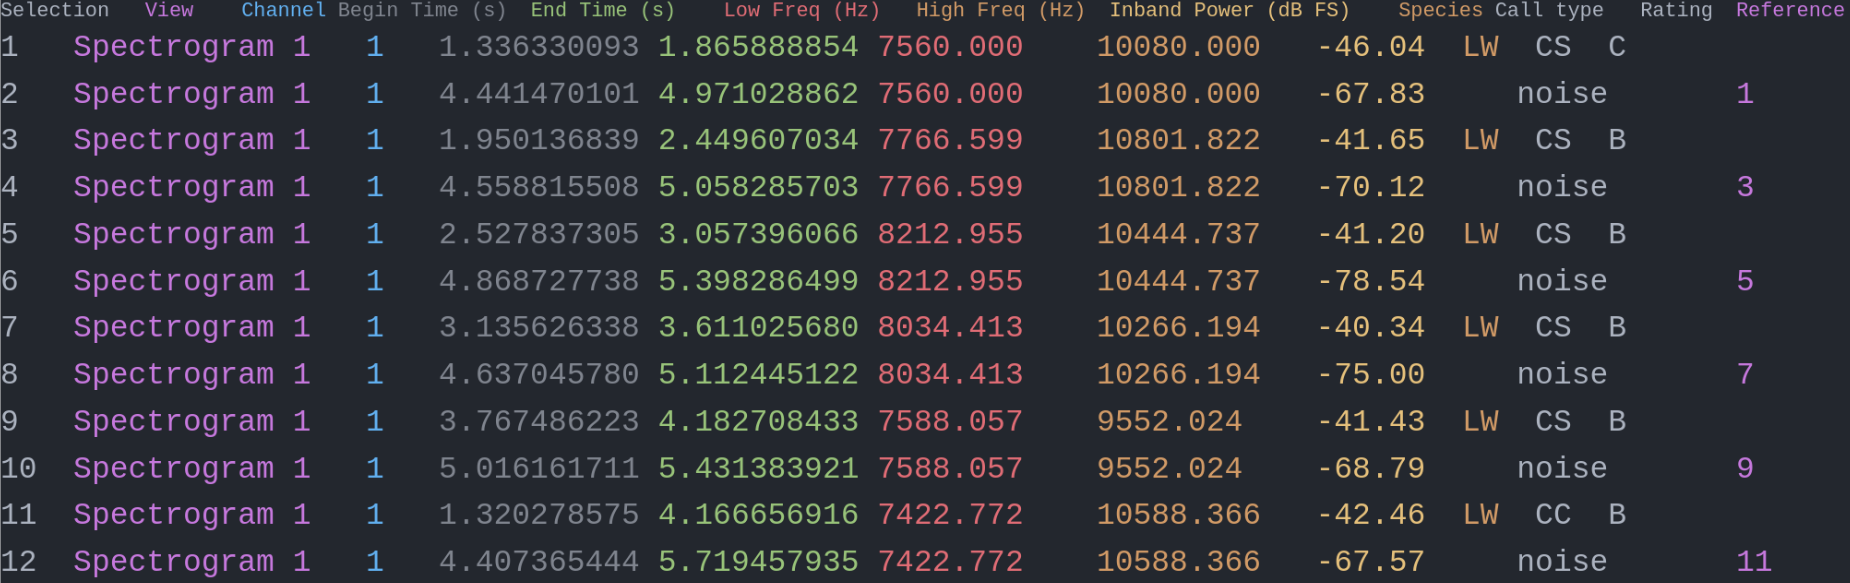
\includegraphics[width=0.95\textwidth]{capitulos/04_oe1_curacion/figures/image4.png}
    \caption[Archivo de anotaciones de Raven]{Archivo de anotaciones de una grabación, con las columnas
        diferenciadas por color. El formato es un archivo de texto delimitado por
        tabulaciones que Raven lee y escribe directamente.}
    \label{fig:anotaciones-crudas}
\end{figure}

Las anotaciones se crean y editan sobre la grabación en Raven
(Figura~\ref{fig:raven}). El analista dibuja una región rectangular sobre el
espectrograma y el software deriva de ella el rango de frecuencias, los tiempos
de inicio y fin, y la amplitud. Las columnas de especie y tipo de llamada se
escriben a mano, y son justamente las que concentran los problemas descritos a
continuación.

\begin{figure}[htbp]
    \centering
    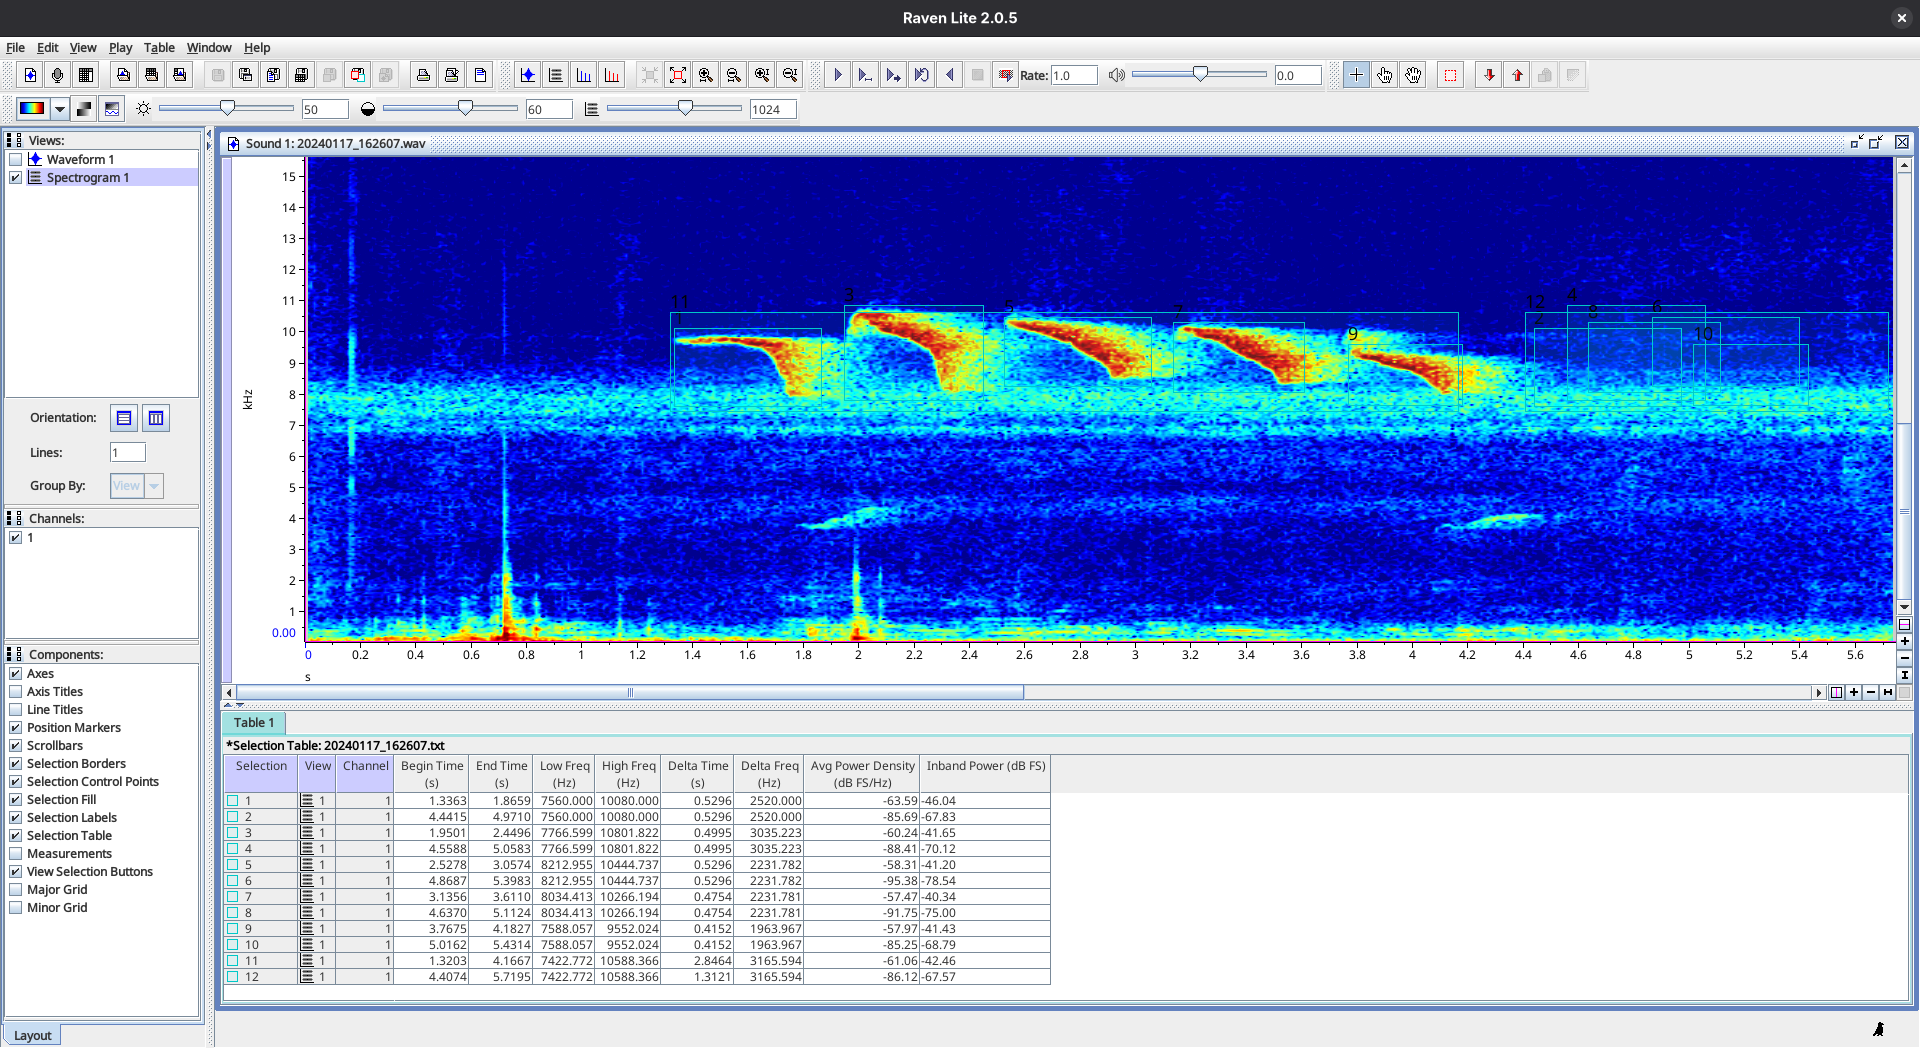
\includegraphics[width=0.92\textwidth]{capitulos/04_oe1_curacion/figures/image5.png}
    \caption[Raven con una grabación anotada]{Raven durante el procesamiento de una grabación junto con sus
        anotaciones. Cada caja del espectrograma corresponde a una fila del archivo
        de la Figura~\ref{fig:anotaciones-crudas}.}
    \label{fig:raven}
\end{figure}

\subsection{Defectos detectados}

Un análisis exploratorio sobre el conjunto reveló cinco problemas que impiden
usar el material directamente para entrenamiento.

\rotulo{Inconsistencias de etiquetado.} Una misma clase aparece escrita de
múltiples formas. El prototipo inicial de este trabajo, restringido a la sílaba
de contacto del tamarino de Weddell, ya encontró en la columna de tipo de llamada
el conjunto de valores distintos
\texttt{\{CS, CS\char32, CS\char32\char32\char32\char32\char32\char32 A, contact
    syllable, CC, contact call, noise, noise\char32\char32\char32, noise|, noises,
    AA, A, B, C, TA\}}: cuatro grafías para una única clase, tres para el descarte
por ruido y un encabezado de columna que unas veces es \texttt{Call type} y otras
\texttt{Call Type}. Las Figuras~\ref{fig:etiquetas-especie}
y~\ref{fig:etiquetas-tipo} muestran los valores únicos encontrados en cada una de
las dos columnas manuales sobre el corpus completo.

\begin{figure}[htbp]
    \centering
    \begin{minipage}[t]{0.46\textwidth}
        \centering
        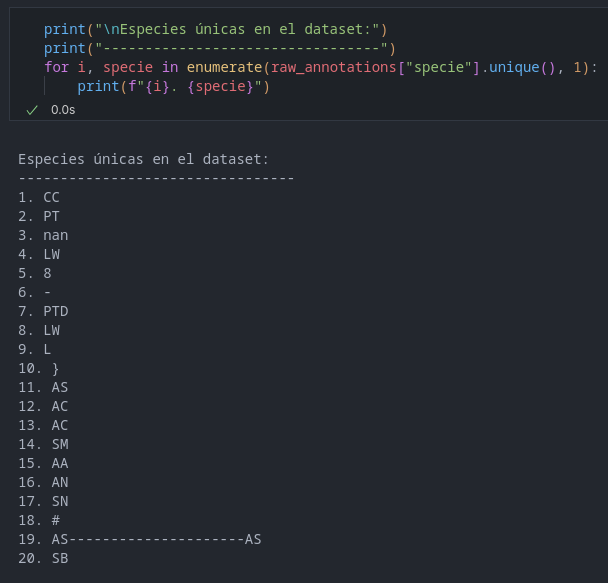
\includegraphics[width=\textwidth]{capitulos/04_oe1_curacion/figures/image6.png}
        \caption{Etiquetas únicas encontradas en la columna de especie.}
        \label{fig:etiquetas-especie}
    \end{minipage}\hfill
    \begin{minipage}[t]{0.46\textwidth}
        \centering
        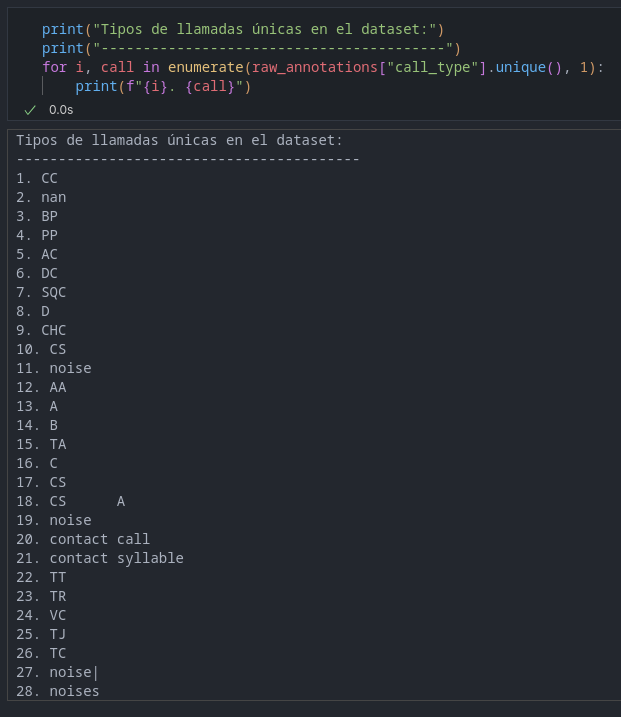
\includegraphics[width=\textwidth]{capitulos/04_oe1_curacion/figures/image7.png}
        \caption{Etiquetas únicas encontradas en la columna de tipo de llamada.}
        \label{fig:etiquetas-tipo}
    \end{minipage}
\end{figure}

\rotulo{Integridad de los archivos.} La carga automatizada de las grabaciones
produce advertencias sobre archivos de audio dañados
(Figura~\ref{fig:advertencias}), que interrumpen el proceso si no se manejan de
forma explícita. La corrupción se manifiesta como bloques de ceros en la señal y
admite grados: la Figura~\ref{fig:corrupcion-leve} muestra un caso leve y la
Figura~\ref{fig:corrupcion-alta} uno en el que la mayor parte del archivo es
inutilizable. El origen probable son cortes durante la transferencia o fallos del
medio de almacenamiento.

\begin{figure}[htbp]
    \centering
    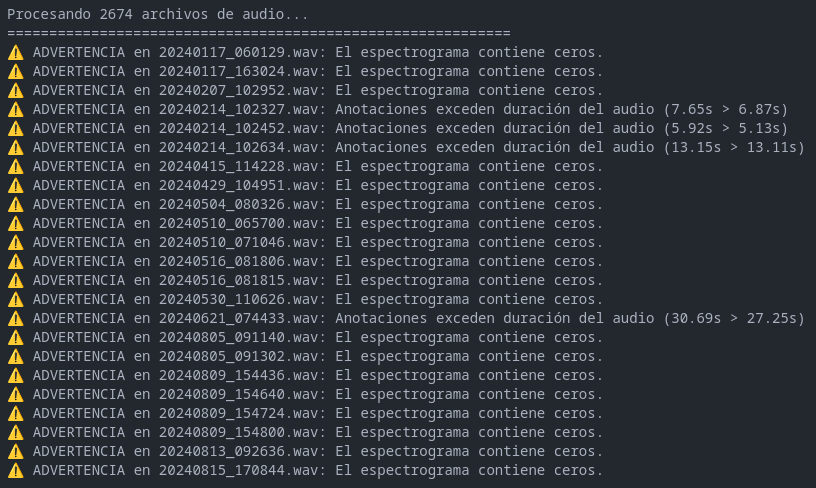
\includegraphics[width=0.85\textwidth]{capitulos/04_oe1_curacion/figures/image8.png}
    \caption{Advertencias emitidas durante la carga automatizada de las
        grabaciones.}
    \label{fig:advertencias}
\end{figure}

\begin{figure}[htbp]
    \centering
    \begin{minipage}[t]{0.48\textwidth}
        \centering
        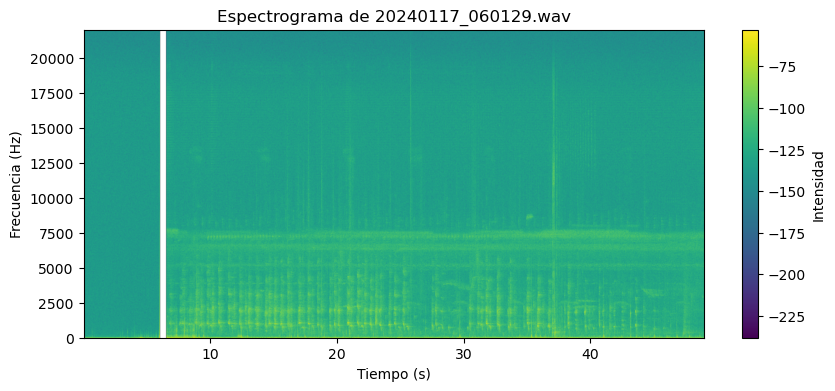
\includegraphics[width=\textwidth]{capitulos/04_oe1_curacion/figures/image9.png}
        \caption{Grabación con corrupción leve}
        \label{fig:corrupcion-leve}
    \end{minipage}\hfill
    \begin{minipage}[t]{0.48\textwidth}
        \centering
        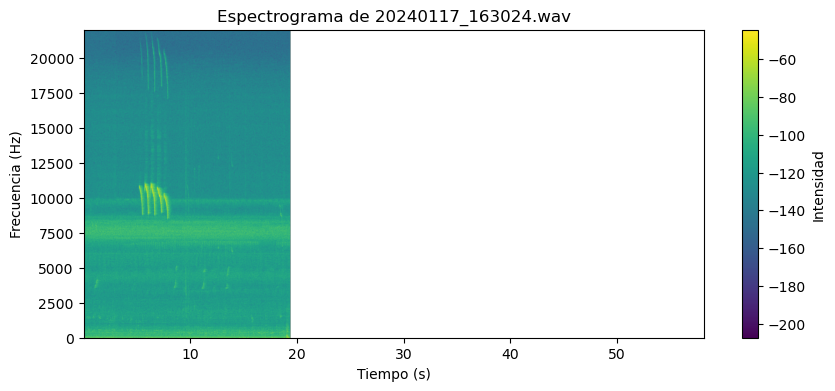
\includegraphics[width=\textwidth]{capitulos/04_oe1_curacion/figures/image10.png}
        \caption{Grabación con corrupción severa}
        \label{fig:corrupcion-alta}
    \end{minipage}
\end{figure}

\rotulo{Discrepancias entre especie y carpeta.} La etiqueta de especie escrita en
la anotación no siempre coincide con el código de la carpeta contenedora, lo que
obliga a decidir cuál de las dos fuentes prevalece antes de consolidar nada.

\rotulo{Frecuencias por encima de Nyquist.} Algunas cajas declaran una frecuencia
superior mayor que el límite de Nyquist de la señal (22\,050\,Hz a 44,1\,kHz de
muestreo), un valor que no puede corresponder a energía observable en la
grabación.

\rotulo{Variabilidad en la unidad de análisis.} La granularidad de las
anotaciones no es uniforme. En unos casos el analista etiquetó sílabas
individuales y en otros delimitó una secuencia completa con una sola caja. No se
trata de un error de anotación sino de la manifestación directa del anidamiento
jerárquico de las unidades acústicas \citep{kershenbaum_acoustic_2016} descrito en el
Capítulo~\ref{cap:marco}; la subsección~\ref{sec:silabas} lo cuantifica.

\subsection{Composición del conjunto curado}

Tras aplicar el protocolo de la sección~\ref{sec:protocolo}, el conjunto queda en
\textbf{19\,042 anotaciones sobre ocho especies, repartidas en 57 pares
    distintos de especie y tipo de llamada}. De esos 57 pares, 41 pertenecen al
vocabulario declarado para el dominio y concentran 18\,714 anotaciones; los 16
restantes, que suman 328 registros (el 1,7\,\%), quedan fuera del vocabulario y se
marcan para revisión en lugar de descartarse en silencio. La
Tabla~\ref{tab:vocab-especie} resume el reparto por especie.

\begin{table}[htbp]
    \centering
    \small
    \begin{threeparttable}
        \caption{Composición del vocabulario curado por especie}
        \label{tab:vocab-especie}
        \begin{tabular}{@{}L{4.9cm}crrcr@{}}
            \toprule
                                           &               & \multicolumn{2}{c}{\textbf{En vocabulario}} & \multicolumn{2}{c}{\textbf{Experimento}}                                        \\
            \cmidrule(lr){3-4}\cmidrule(lr){5-6}
            \textbf{Especie}               & \textbf{Cód.} & \thead{Tipos}                               & \thead{Anotaciones}                      & \thead{Clases} & \thead{Anotaciones} \\
            \midrule
            \textit{Leontocebus weddelli}  & LW            & 11                                          & 4\,123                                   & 5              & 3\,492              \\
            \textit{Sapajus macrocephalus} & SM            & 8                                           & 3\,605                                   & 5              & 3\,395              \\
            \textit{Alouatta sara}         & AS            & 2                                           & 3\,310                                   & 2              & 3\,310              \\
            \textit{Ateles chamek}         & AC            & 6                                           & 3\,081                                   & 4              & 3\,017              \\
            \textit{Saimiri boliviensis}   & SB            & 5                                           & 2\,326                                   & 4              & 2\,277              \\
            \textit{Plecturocebus toppini} & PT            & 5                                           & 1\,156                                   & 2              & 1\,030              \\
            \textit{Aotus azarae}          & AA            & 3                                           & 1\,084                                   & 3              & 1\,084              \\
            \textit{Cebus cuscinus}        & CC            & 1                                           & 29                                       & 0              & N/D                 \\
            \midrule
            \textbf{Total}                 &               & \textbf{41}                                 & \textbf{18\,714}                         & \textbf{25}    & \textbf{17\,605}    \\
            \bottomrule
        \end{tabular}
        \begin{tablenotes}[flushleft]
            \footnotesize
            \item Las 328 anotaciones restantes hasta 19\,042 corresponden a los
            16 pares fuera de vocabulario, marcados para revisión.
            \item Los cuatro tipos de trino de LW cuentan como cuatro entradas
            del vocabulario y como una sola clase del experimento, por la fusión
            que justifica la sección~\ref{sec:seleccion}.
        \end{tablenotes}
    \end{threeparttable}
\end{table}

Dos propiedades de esa tabla gobiernan el resto del capítulo. La primera es que
\textbf{el vocabulario es desigual entre especies}: LW aporta once tipos de
llamada distintos sobre 4\,103 anotaciones, mientras que CC aporta un único tipo
con 29. La segunda es que \textbf{la distribución dentro de una especie es tan
    sesgada como la distribución entre especies}: en SM, el par \texttt{sm/acc}
cuenta con 8 anotaciones frente a las 2\,040 de \texttt{sm/cc}, un factor de
255$\times$ dentro de un mismo repertorio. La cola es
larga: los diez pares mayores concentran el 74\,\% de las 19\,042 anotaciones y
el resto se reparte hasta pares con una sola.

\begin{figure}[htbp]
    \centering
    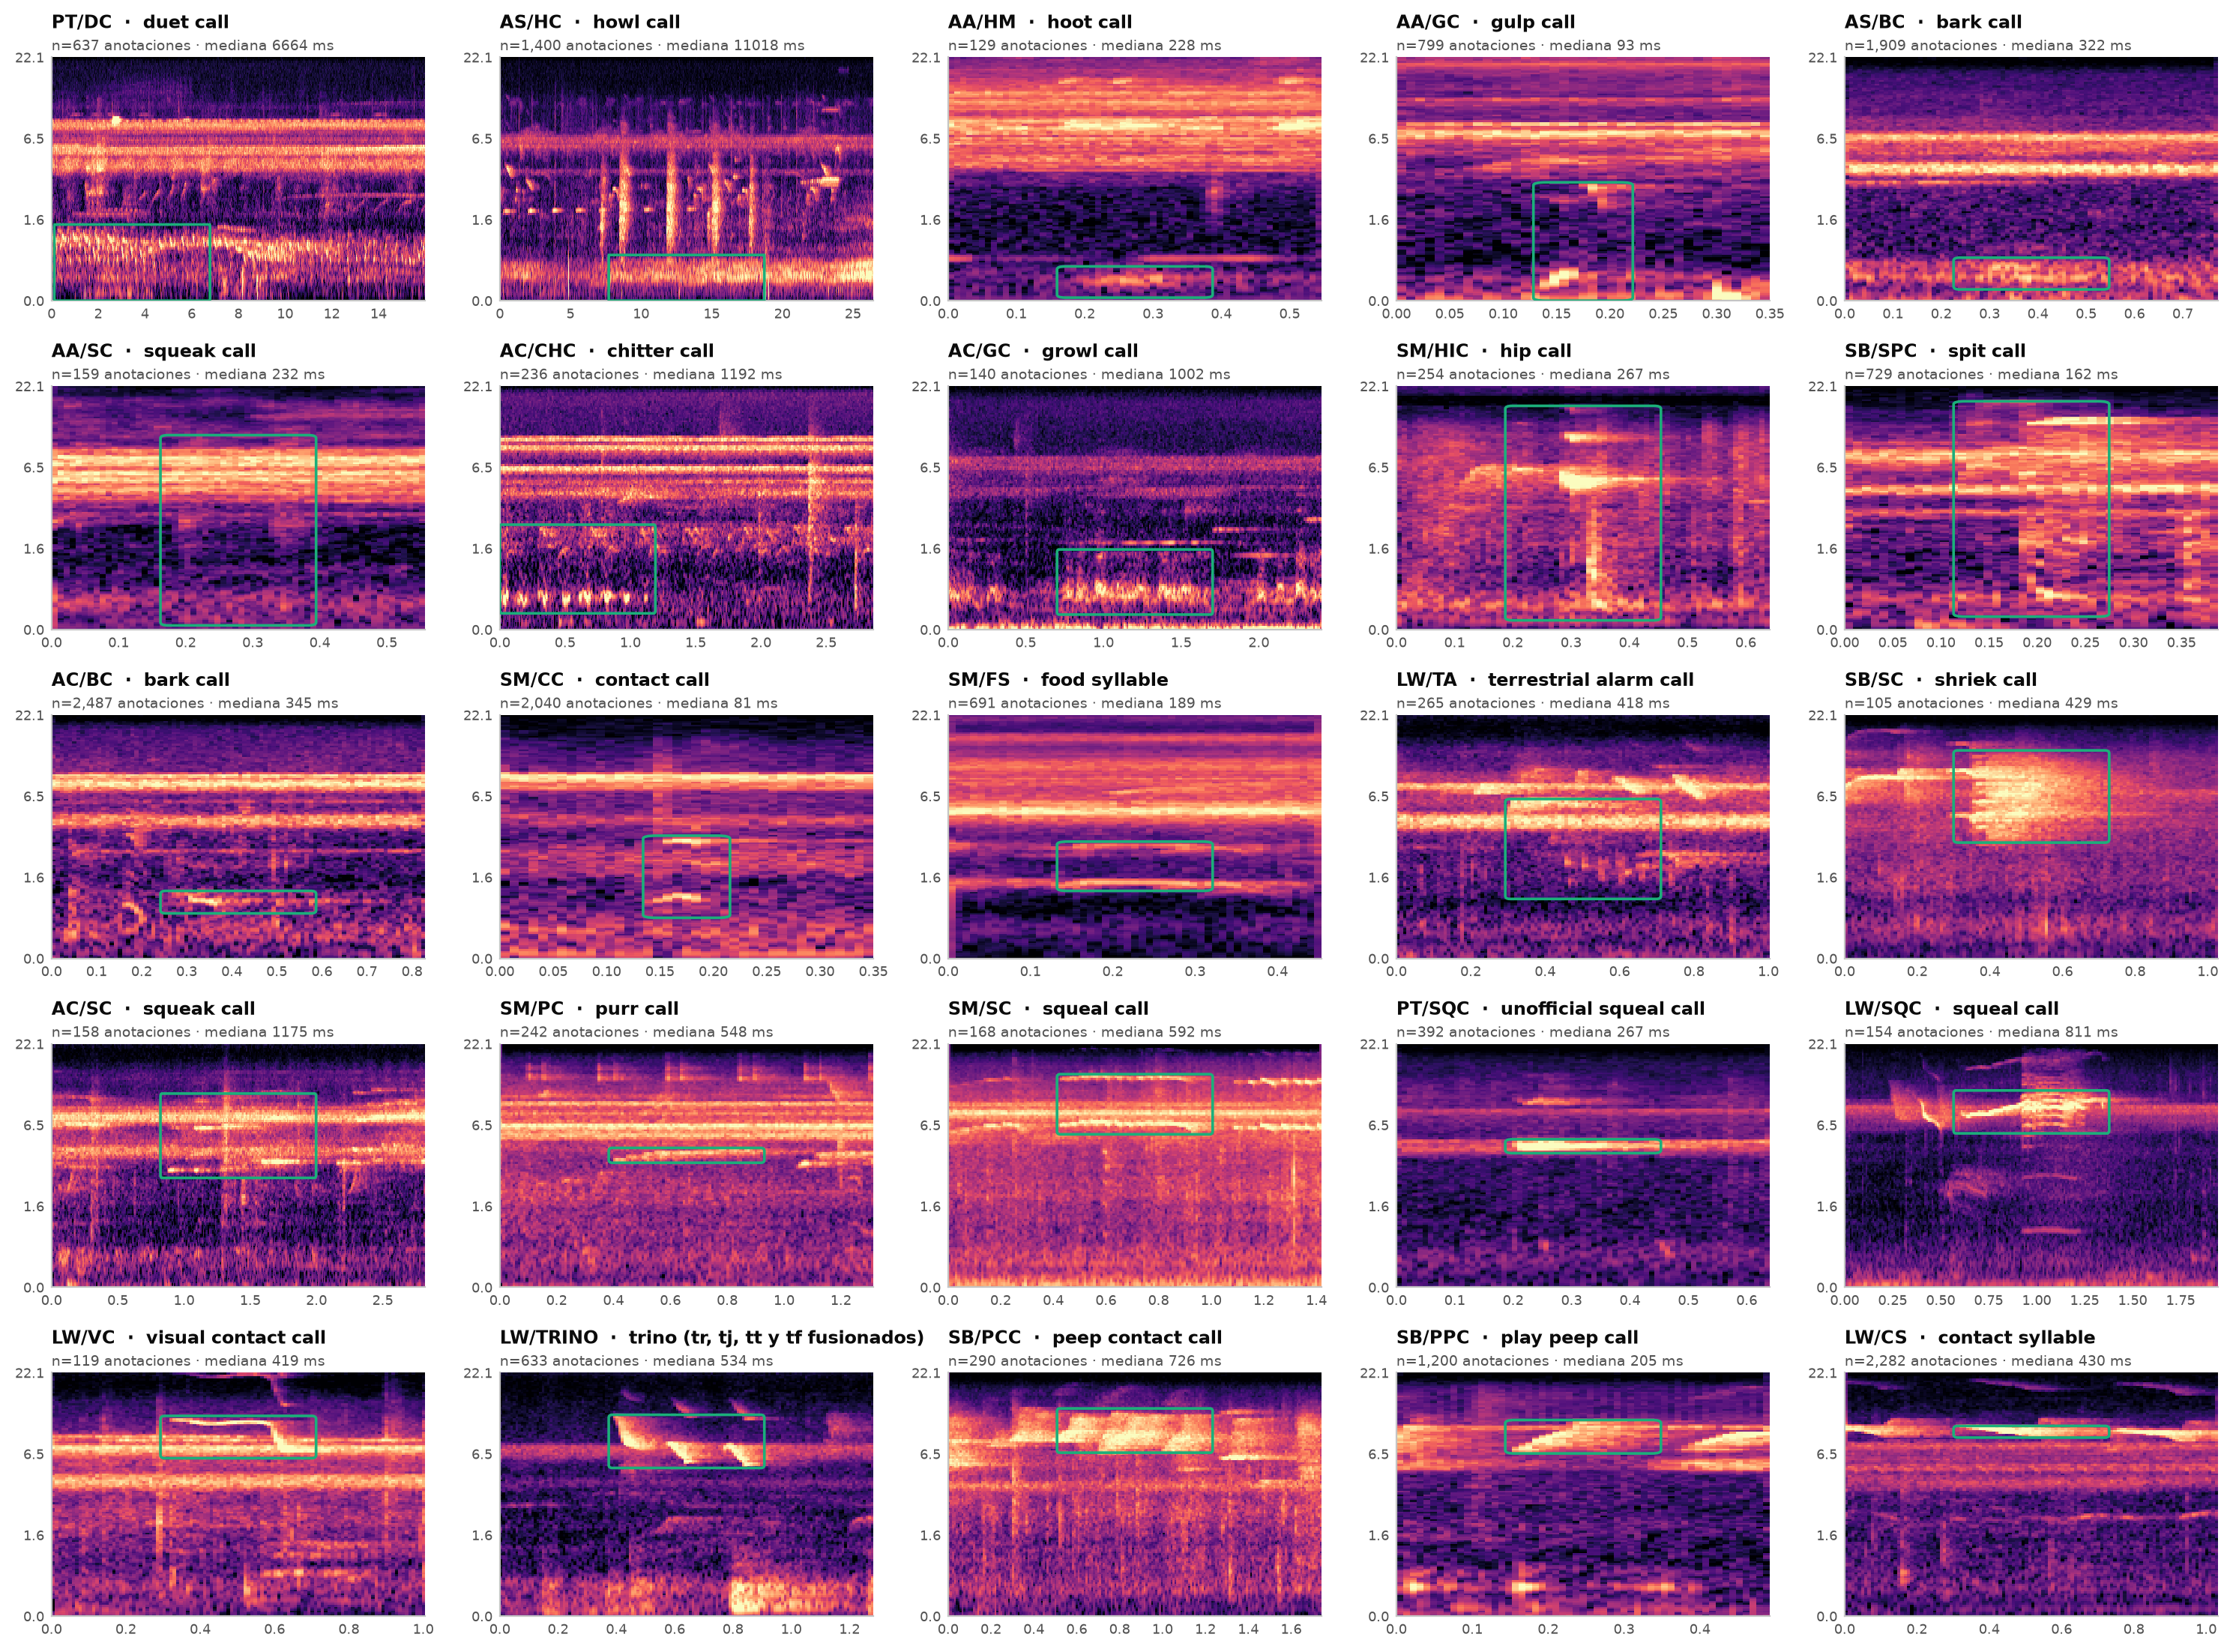
\includegraphics[width=\textwidth]{capitulos/04_oe1_curacion/figures/call_gallery.png}
    \caption{Galería de llamadas.}
    \label{fig:call-gallery}
\end{figure}

\subsection{Geometría de los eventos}
\label{sec:geometria}

Las llamadas anotadas son extraordinariamente desiguales en tamaño, y ese hecho
condiciona todas las decisiones de diseño que siguen. La
Tabla~\ref{tab:geometria} lo mide sobre las 19\,042 anotaciones.

\begin{table}[htbp]
    \centering
    \caption{Variación de tamaño de las llamadas anotadas}
    \label{tab:geometria}
    \small
    \begin{tabular}{@{}L{4.0cm}rrr@{}}
        \toprule
                       & \thead{Mínimo} & \thead{Máximo} & \thead{Razón}           \\
        \midrule
        Duración       & 0,034\,s       & 73,3\,s        & \textbf{2\,134$\times$} \\
        Ancho de banda & 224\,Hz        & 21\,784\,Hz    & 97$\times$              \\
        \bottomrule
    \end{tabular}
\end{table}

La llamada más larga dura más de dos mil veces lo que la más corta. La magnitud
se aprecia mejor por comparación: en COCO, la colección de imágenes con la que se
evalúan habitualmente los detectores de objetos \citep{lin_2014}, los objetos
mayores superan a los menores en un factor de entre 10 y 100. El problema que
enfrenta este detector es, en ese eje, un orden de magnitud más severo que aquel
para el que se diseñaron las arquitecturas que hereda.

La consecuencia inmediata es que \textbf{ninguna longitud de ventana única sirve
    para todas las clases}: una ventana capaz de contener un aullido de 73\,s es
demasiado gruesa para resolver un chirrido de 34\,ms. La
sección~\ref{sec:ventaneo} documenta el compromiso adoptado y lo que cuesta.

La Tabla~\ref{tab:class-geometry} sitúa cada clase en duración y en banda de
frecuencia, y hace visibles dos efectos a la vez.
Las \textbf{especies se separan en buena medida por banda}: AS ocupa
aproximadamente entre 25 y 1\,410\,Hz (percentiles 1 y 99), mientras que
\texttt{lw/cs} nunca aparece anotada por debajo de 3\,687\,Hz. Los \textbf{tipos
    de llamada dentro de una misma especie no se separan}: en LW, la familia de
trinos junto con \texttt{vc} y \texttt{cs} comparten banda y duración casi por
completo.

\begin{table}[htbp]
    \centering
    \begin{threeparttable}
        \caption[Geometría de las clases]{Duración, banda de frecuencia y ancho de banda de cada
            clase, ordenadas por duración mediana descendente}
        \label{tab:class-geometry}
        \footnotesize
        \begin{tabular}{@{}L{1.7cm}L{3.4cm}L{3.3cm}R{2.0cm}@{}}
            \toprule
            \textbf{Clase} & \thead[l]{Duración\\mediana (s)} & \thead[l]{Banda de\\frecuencia (Hz)} & \thead[l]{Ancho de\\banda (Hz)} \\
            \midrule
            \texttt{as/hc}    & 11,0\,s [7,1--15,9]   & 48--769\,Hz          & 727\,Hz    \\
            \texttt{pt/dc}    & 6,7\,s [4,8--9,5]     & 25--1\,474\,Hz       & 1\,409\,Hz \\
            \texttt{ac/chc}   & 1,2\,s [0,86--1,6]    & 192--3\,363\,Hz      & 3\,178\,Hz \\
            \texttt{ac/sc}    & 1,2\,s [0,87--1,4]    & 2\,640--10\,726\,Hz  & 8\,135\,Hz \\
            \texttt{ac/gc}    & 1,0\,s [0,66--1,9]    & 198--1\,465\,Hz      & 1\,276\,Hz \\
            \texttt{lw/sqc}   & 0,81\,s [0,60--1,0]   & 5\,035--12\,912\,Hz  & 7\,728\,Hz \\
            \texttt{sb/pcc}   & 0,73\,s [0,50--1,1]   & 6\,531--11\,749\,Hz  & 4\,961\,Hz \\
            \texttt{sm/sc}    & 0,59\,s [0,37--0,82]  & 3\,387--10\,678\,Hz  & 6\,878\,Hz \\
            \texttt{sm/pc}    & 0,55\,s [0,40--0,82]  & 2\,806--4\,435\,Hz   & 1\,542\,Hz \\
            \texttt{lw/trino} & 0,53\,s [0,35--0,73]  & 5\,740--11\,126\,Hz  & 5\,455\,Hz \\
            \texttt{lw/cs}    & 0,43\,s [0,34--0,50]  & 8\,037--10\,215\,Hz  & 2\,101\,Hz \\
            \texttt{sb/sc}    & 0,43\,s [0,35--0,58]  & 2\,534--15\,464\,Hz  & 13\,243\,Hz \\
            \texttt{lw/ta}    & 0,42\,s [0,31--0,55]  & 1\,545--6\,883\,Hz   & 5\,152\,Hz \\
            \texttt{lw/vc}    & 0,42\,s [0,33--0,49]  & 5\,338--8\,808\,Hz   & 3\,497\,Hz \\
            \texttt{ac/bc}    & 0,35\,s [0,24--0,50]  & 374--2\,616\,Hz      & 2\,235\,Hz \\
            \texttt{as/bc}    & 0,32\,s [0,26--0,40]  & 105--668\,Hz         & 567\,Hz    \\
            \texttt{pt/sqc}   & 0,27\,s [0,24--0,31]  & 4\,338--5\,083\,Hz   & 666\,Hz    \\
            \texttt{sm/hic}   & 0,27\,s [0,19--0,36]  & 249--4\,927\,Hz      & 4\,649\,Hz \\
            \texttt{aa/sc}    & 0,23\,s [0,21--0,27]  & 107--13\,147\,Hz     & 12\,792\,Hz \\
            \texttt{aa/hm}    & 0,23\,s [0,19--0,27]  & 66--529\,Hz          & 452\,Hz    \\
            \texttt{sb/ppc}   & 0,20\,s [0,14--0,29]  & 7\,010--11\,251\,Hz  & 3\,924\,Hz \\
            \texttt{sm/fs}    & 0,19\,s [0,15--0,26]  & 1\,210--2\,438\,Hz   & 1\,292\,Hz \\
            \texttt{sb/spc}   & 0,16\,s [0,13--0,22]  & 248--15\,933\,Hz     & 15\,602\,Hz \\
            \texttt{aa/gc}    & 0,09\,s [0,08--0,12]  & 97--3\,076\,Hz       & 2\,859\,Hz \\
            \texttt{sm/cc}    & 0,08\,s [0,06--0,11]  & 523--3\,606\,Hz      & 3\,066\,Hz \\
            \bottomrule
        \end{tabular}
        \begin{tablenotes}[flushleft]
            \footnotesize
            \item RIC: rango intercuartílico (percentiles 25--75) de la duración.
            La banda de frecuencia es [mediana de $f_{\min}$, mediana de
            $f_{\max}$] por clase; el ancho de banda es la mediana de
            $f_{\max} - f_{\min}$ calculada anotación por anotación, no la resta
            de las medianas de la columna anterior. Calculado sobre las 17\,605
            anotaciones del subconjunto de experimento (Tabla~\ref{tab:clases-experimento})
            con \texttt{notebooks/dataset\_report.ipynb}.
        \end{tablenotes}
    \end{threeparttable}
\end{table}

Esa disociación tiene una consecuencia metodológica directa, y es la que sostiene
el protocolo de evaluación del Capítulo~\ref{cap:deteccion}: si la geometría
distingue especies pero no tipos de llamada, entonces \emph{localizar} y
\emph{etiquetar} son problemas de dificultad distinta y no deben puntuarse con
una sola cifra. De ahí que la detección se entrene de forma agnóstica a la clase
y la clasificación se evalúe por separado.

La Figura~\ref{fig:facets} desglosa la geometría par por par y revela un problema distinto del desbalance:
\texttt{ac/bc} (coeficiente de variación del ancho de banda 0,60) y
\texttt{sm/fs} (0,63) se parten cada uno en dos nubes claramente separadas en el
plano duración\,$\times$\,ancho de banda, mientras que \texttt{sb/ppc} (0,47) es
una única mancha difusa. Que una etiqueta cubra dos nubes disjuntas sugiere que
agrupa dos variantes de llamada que el vocabulario actual no distingue. Es un
hallazgo sobre el esquema de anotación, no sobre el modelo. Son, además, las
clases con peor \textit{recall} en la evaluación del
Capítulo~\ref{cap:deteccion}.

\begin{figure}[htbp]
    \centering
    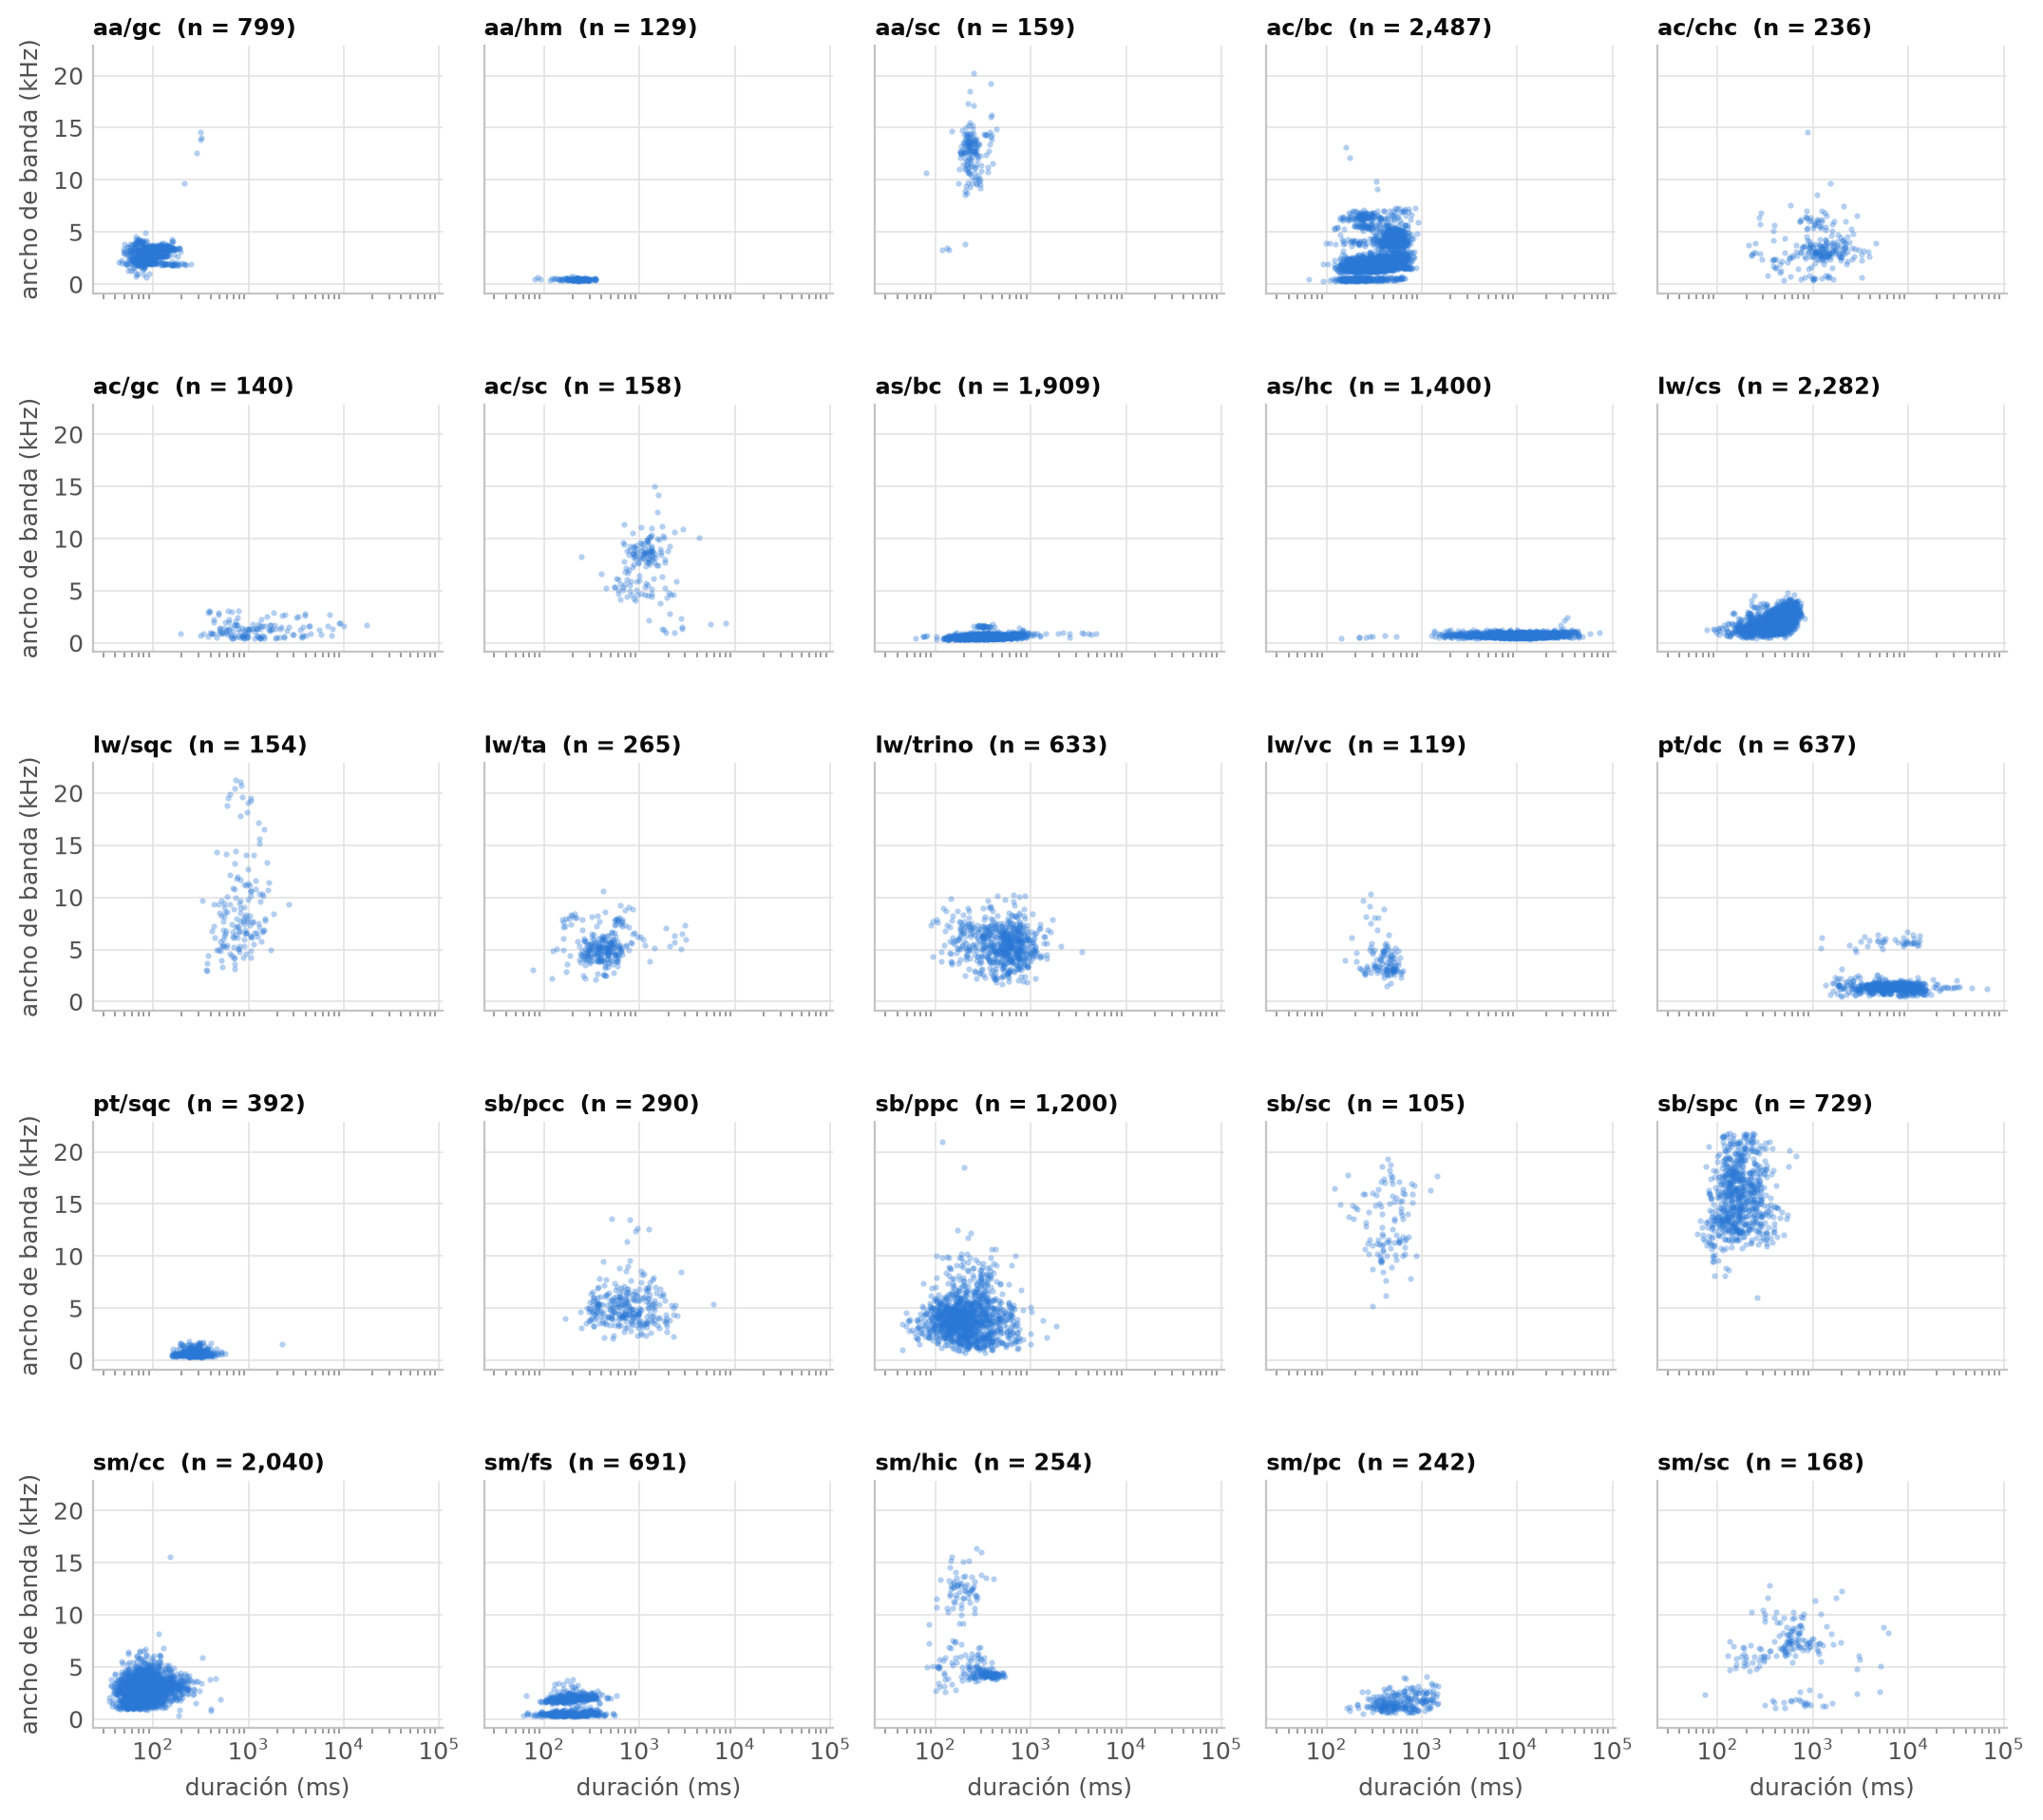
\includegraphics[height=0.80\textheight]{capitulos/04_oe1_curacion/figures/class_geometry_facets.png}
    \caption[Duración frente a ancho de banda]{Duración frente a ancho de banda, un panel por par del
        vocabulario curado. En gris, todas las clases; en color, la del panel. Las
        nubes partidas de \texttt{ac/bc} y \texttt{sm/fs} indican una etiqueta
        única que cubre dos variantes de llamada.}
    \label{fig:facets}
\end{figure}

\subsection{Sílabas y frases}
\label{sec:silabas}

Una \emph{frase} es una secuencia de \emph{sílabas}, y los expertos anotan ambas:
el 94,2\,\% de las frases \texttt{lw/cc} contienen al menos una sílaba
\texttt{lw/cs}, y el 96,8\,\% de las frases \texttt{sm/fc} contienen una sílaba
\texttt{sm/fs}. El mismo tramo de audio lleva, por tanto, una caja grande y
varias cajas pequeñas dentro de ella.

El detector no puede representar esa relación. Devuelve una lista plana de cajas,
y el emparejamiento durante el entrenamiento asocia cada anotación verdadera con
exactamente una predicción, sin manera de expresar que ``esta caja contiene a
aquella''. Conservar ambos niveles equivaldría a pedir al modelo que informe dos
veces el mismo sonido, como si fueran dos eventos no relacionados superpuestos.
Es la consecuencia operativa del anidamiento jerárquico que
\citet{kershenbaum_acoustic_2016} describen como propiedad general de las unidades
acústicas animales: una secuencia de unidades puede ella misma considerarse una
unidad. Las dos clases de frase se excluyen, en consecuencia, antes del
entrenamiento.

\begin{figure}[htbp]
    \centering
    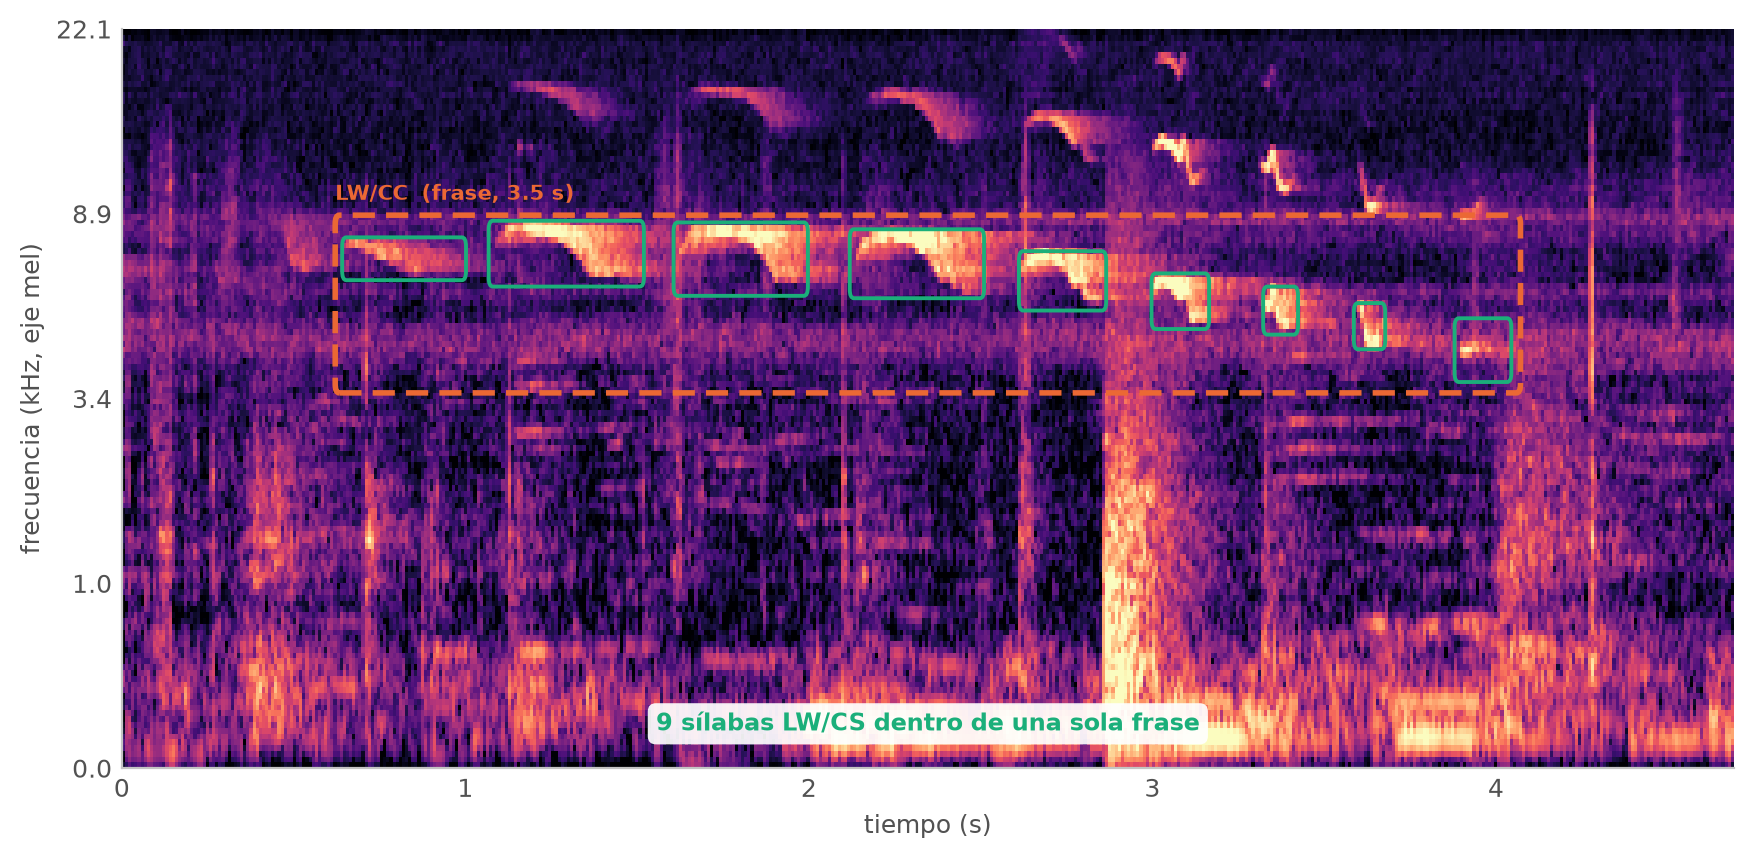
\includegraphics[width=0.92\textwidth]{capitulos/04_oe1_curacion/figures/nesting_phrase.png}
    \caption{Anidamiento frase-sílaba.}
    \label{fig:nesting-phrase}
\end{figure}

\section{Protocolo de curación y estandarización documentado (RE1.1)}
\label{sec:re11}
\label{sec:protocolo}

El protocolo se implementa como un \textit{pipeline} programático, no como una
corrección manual del material recibido. La distinción importa: un protocolo
ejecutable puede volver a aplicarse sobre los datos primarios cada vez que sus
reglas cambian, y deja registro de qué se descartó y por qué.

\begin{figure}[htbp]
    \centering
    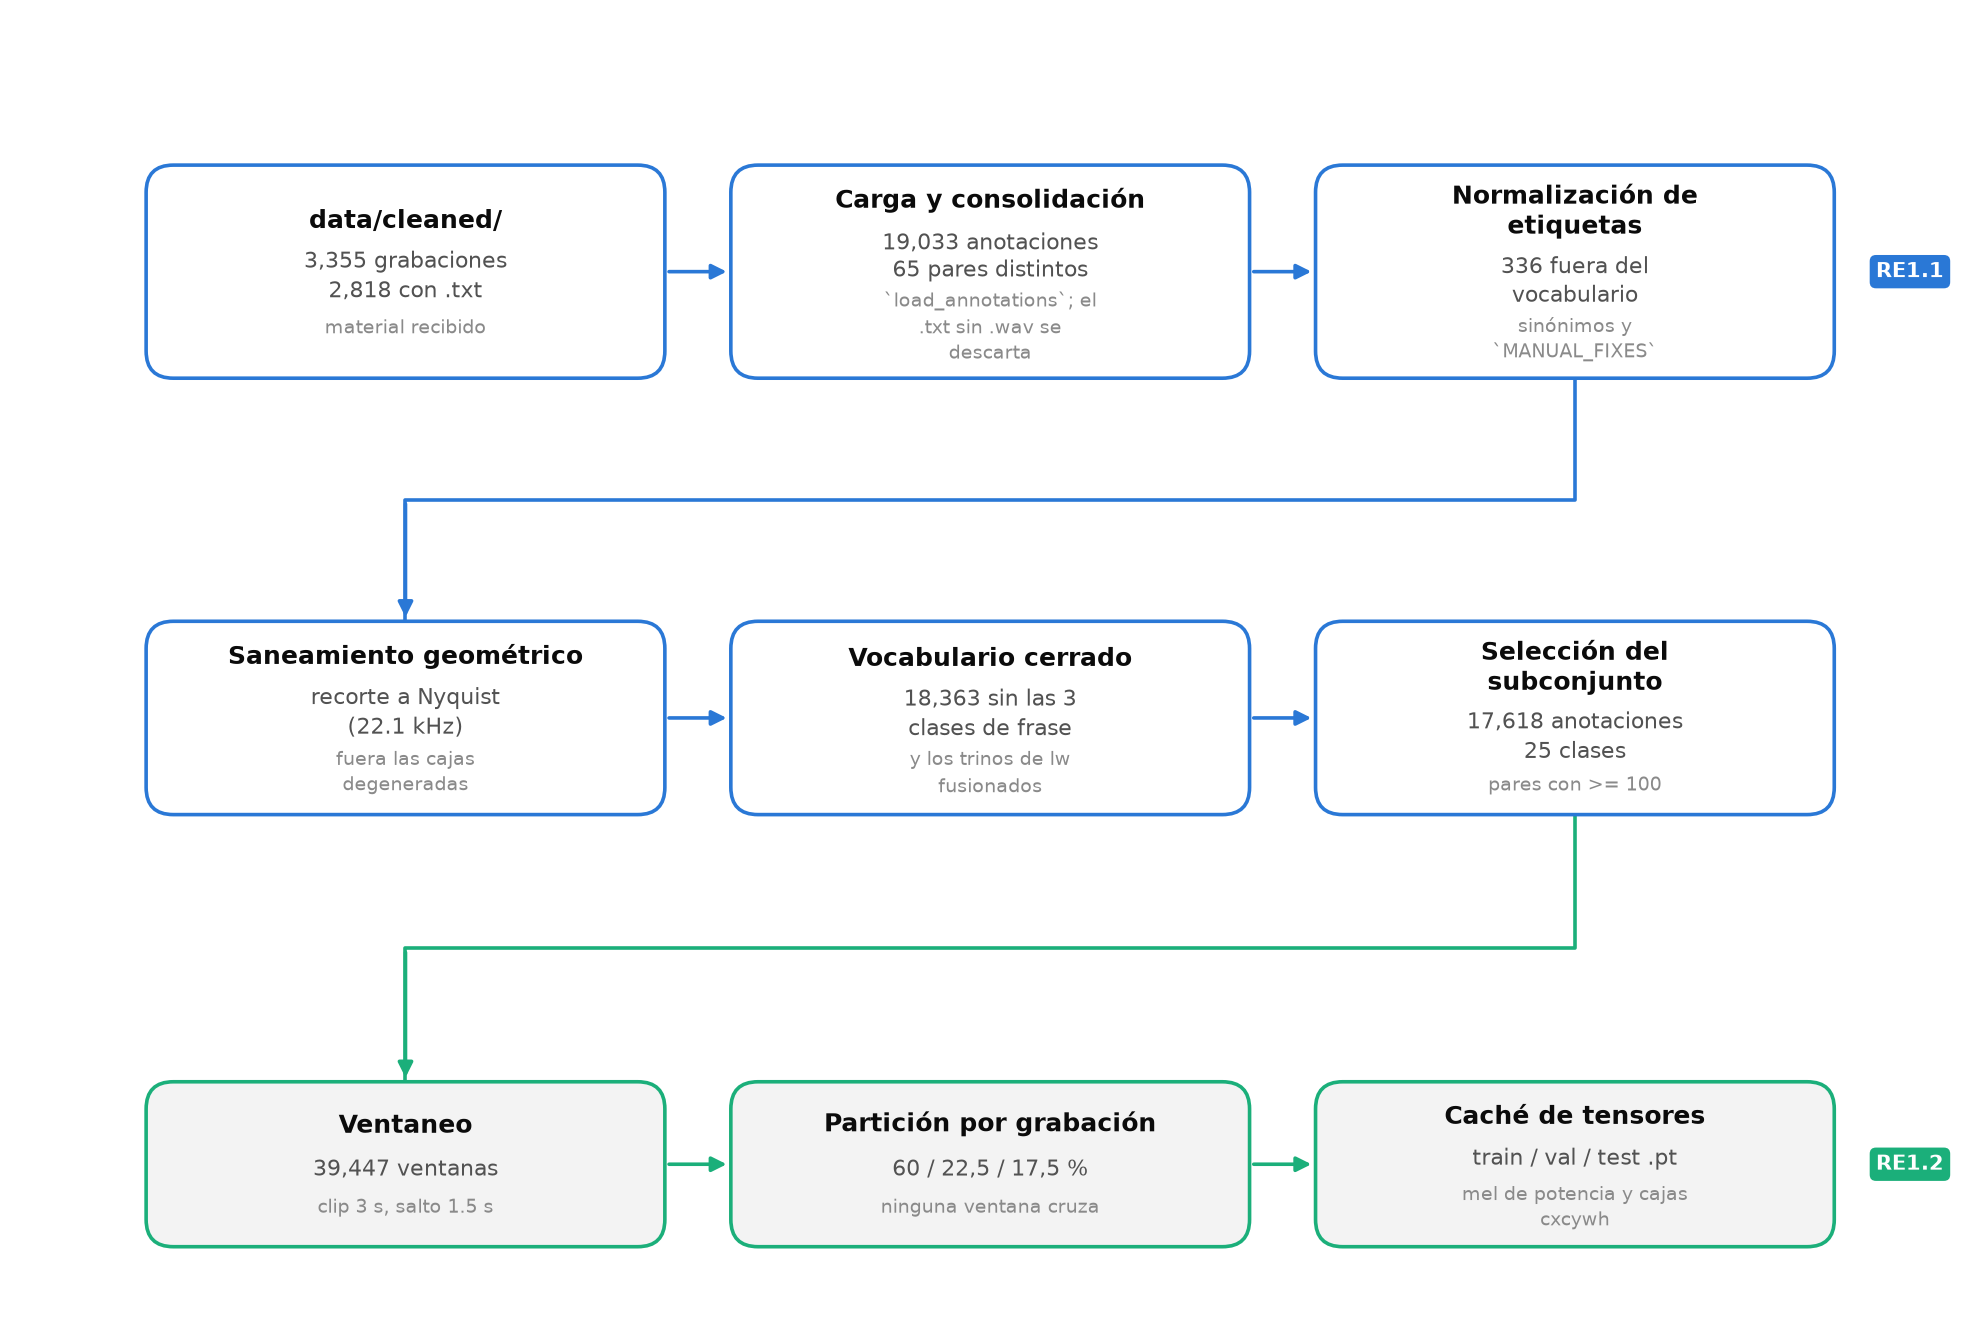
\includegraphics[width=\textwidth]{capitulos/04_oe1_curacion/figures/curation_pipeline.png}
    \caption{Pipeline de curación.}
    \label{fig:curation-pipeline}
\end{figure}

\subsection{Carga y consolidación}

El primer paso recorre la estructura de directorios, lee cada archivo de
anotación y los unifica en una única tabla. Para cada archivo:

\begin{description}
    \item[Emparejamiento con el audio.] Solo se carga el archivo de anotación que
          tiene una grabación homónima junto a él. Un archivo de texto huérfano no
          aporta nada entrenable y su presencia suele indicar un error de transferencia.

    \item[Normalización de nombres de columna.] Los encabezados originales se
          convierten a un formato programático uniforme; \texttt{Begin Time (s)} pasa a
          \texttt{begin\_time\_s}, y de forma análoga el resto. Esto resuelve de una vez
          la alternancia entre \texttt{Call type} y \texttt{Call Type} observada en el
          material crudo.

    \item[Descarte de columnas no utilizadas.] Se eliminan las columnas de
          selección, vista, canal, referencia y desplazamiento de archivo, que
          corresponden al estado interno de Raven y no al evento.

    \item[Enriquecimiento con metadatos.] Se añaden la ruta de la grabación de
          origen y el directorio contenedor, que preserva la especie declarada por la
          organización del corpus.
\end{description}

Los errores de lectura se capturan y se registran, de modo que un archivo dañado
o un directorio vacío se omitan sin detener el proceso.

\subsection{Normalización de etiquetas}

Sobre la tabla consolidada se aplican, en este orden, las siguientes reglas.

\begin{description}
    \item[Normalización tipográfica.] Toda etiqueta se reduce a minúsculas y a
          caracteres alfanuméricos separados por guion bajo. Este único paso absorbe la
          mayoría de las variantes observadas, como espacios en blanco al final,
          mayúsculas inconsistentes y caracteres residuales, sin necesidad de
          enumerarlas.

    \item[Mapa de sinónimos.] Un diccionario explícito unifica las variantes que
          la normalización tipográfica no captura, por ser errores de escritura o
          abreviaturas alternativas y no diferencias de formato: \texttt{noises} a
          \texttt{noise}, \texttt{cs\_a} a \texttt{cs}, \texttt{whinnie} a
          \texttt{whc}, \texttt{tca} y \texttt{tac} a \texttt{ta}, \texttt{contact} a
          \texttt{cc}, \texttt{chcj} a \texttt{chc}, \texttt{php} a \texttt{phc},
          \texttt{sqr} a \texttt{sqc}, y \texttt{tc} a \texttt{tr}. Al mapa se suma, por
          especie, la traducción del nombre legible del tipo de llamada a su código
          \texttt{contact syllable} a \texttt{cs}, de modo que las anotaciones
          escritas en prosa converjan con las escritas en código.

    \item[Descarte de ruido.] Las anotaciones cuyo tipo de llamada, ya
          normalizado, es \texttt{noise} se eliminan: marcan la ausencia de evento, no
          un evento.

    \item[Corrección de pares imposibles.] Un pequeño conjunto de correcciones
          explícitas resuelve pares que no existen en el repertorio de la especie y
          cuya intención es inequívoca; por ejemplo, \texttt{aa/hc} se corrige a
          \texttt{aa/hm}, dado que AA no tiene llamada de aullido pero sí de ululato.
\end{description}

Ante una discrepancia entre la especie escrita en la anotación y el código de la
carpeta contenedora, prevalece la carpeta. El criterio no es arbitrario: el directorio es un dato estructural,
fijado una vez por sesión de campo, mientras que la columna de especie se teclea
en cada fila y es donde se observaron los errores de la
Figura~\ref{fig:etiquetas-especie}.

\subsection{Saneamiento geométrico}

Las coordenadas de la caja se validan de forma independiente de la etiqueta:

\begin{description}
    \item[Recorte a Nyquist.] La frecuencia superior se recorta a 22\,050\,Hz.
          Por encima de ese límite no hay energía observable en una señal muestreada a
          44,1\,kHz, de modo que un valor mayor es un error de anotación y no una
          propiedad del evento.

    \item[Descarte de cajas degeneradas.] Se eliminan las anotaciones de duración
          inferior a 10\,ms y las de ancho de banda nulo o negativo. Una caja sin área
          no define una región y no puede emparejarse con ninguna predicción.

    \item[Características derivadas.] Se calculan la duración y el ancho de banda
          de cada caja, que son las magnitudes sobre las que se construye el análisis de
          la sección~\ref{sec:geometria}.
\end{description}

\subsection{Vocabulario cerrado y selección del subconjunto}
\label{sec:seleccion}

El vocabulario admisible se declara de forma explícita como el conjunto de pares
(especie, tipo de llamada) válidos del dominio, no como aquello que aparezca en
los datos. Cerrar el vocabulario es la respuesta a la condición subyacente S2 del
árbol de problemas: las definiciones de unidad y las etiquetas semánticas varían
ampliamente entre investigadores, incluso dentro de un mismo grupo taxonómico
\citep{kershenbaum_acoustic_2016}, de modo que sin una lista fija la misma señal recibe
etiquetas distintas según quién la anote.

Los pares que caen fuera del vocabulario, 16 pares que suman 328 registros, no se
eliminan: se marcan con una bandera de revisión. La diferencia es deliberada. Un
par fuera de vocabulario puede ser un error de escritura no previsto o un tipo de
llamada legítimo aún no incorporado, y solo el equipo de investigación puede
distinguir uno de otro. Descartarlos en silencio destruiría esa evidencia.

Sobre el vocabulario se recorta el subconjunto de experimento en tres pasos:

\begin{enumerate}[nosep]
    \item \textbf{Exclusión por anidamiento.} Se retiran las dos clases de frase,
          \texttt{lw/cc} (517 anotaciones) y \texttt{sm/fc} (126), por la razón de la
          sección~\ref{sec:silabas}, y \texttt{sb/pcs} (8), que es la misma relación
          frase--sílaba dentro del repertorio de SB.

    \item \textbf{Fusión de los trinos de LW.} Los cuatro tipos de trino
          (\texttt{tr}, 333; \texttt{tj}, 164; \texttt{tt}, 106; \texttt{tf}, 31) se
          reúnen en una única clase \texttt{lw/trino} de 634 anotaciones. El motivo es
          geométrico y proviene de la sección~\ref{sec:geometria}: los cuatro comparten
          banda y duración casi por completo, de modo que mantenerlos separados obliga
          al detector a distinguir lo que la representación no distingue, y reparte
          entre cuatro etiquetas escasas un material que como clase única sí alcanza
          masa suficiente.

    \item \textbf{Umbral de frecuencia.} Se conservan los pares con al menos 100
          anotaciones. Por debajo de ese piso una clase no sostiene ni entrenamiento ni
          evaluación por clase: la más escasa que sobrevive, \texttt{sb/sc} con 105
          anotaciones, aporta apenas 126 cajas de entrenamiento.
\end{enumerate}

El resultado son las \textbf{25 clases y 17\,605 anotaciones} de la
Tabla~\ref{tab:clases-experimento}, el 92,5\,\% del conjunto curado, distribuidas
sobre siete de las ocho especies. El umbral deja fuera 26 pares con 786
anotaciones; de ellos, once pertenecen al vocabulario y suman 466 anotaciones,
entre los que está \texttt{cc/cc}: con 29 registros, la única llamada de CC no
alcanza el piso y esa especie queda fuera del experimento, aunque permanece en el
conjunto curado.

La elección del umbral en 100 y no más arriba es deliberada, y responde a una
tensión que conviene enunciar. Un umbral alto produce un experimento cómodo
—pocas clases, todas abundantes— a costa de dejar sin cubrir la mayor parte del
repertorio documentado: con el piso en 500 anotaciones sobrevivían diez clases,
el 74\,\% del material, y veintinueve tipos de llamada del vocabulario quedaban
sin usar. Bajar el piso a 100 cubre el 92,5\,\% del material y las cinco especies
que antes aportaban una sola clase pasan a aportar entre dos y cinco, al precio
de admitir clases cuyo desempeño estará limitado por su propia escasez y no por
la arquitectura. El Capítulo~\ref{cap:deteccion} lee los resultados por clase con
esa distinción presente, y la Figura~\ref{fig:annotations-per-pair} sitúa el
umbral sobre la distribución completa de pares.

\begin{figure}[htbp]
    \centering
    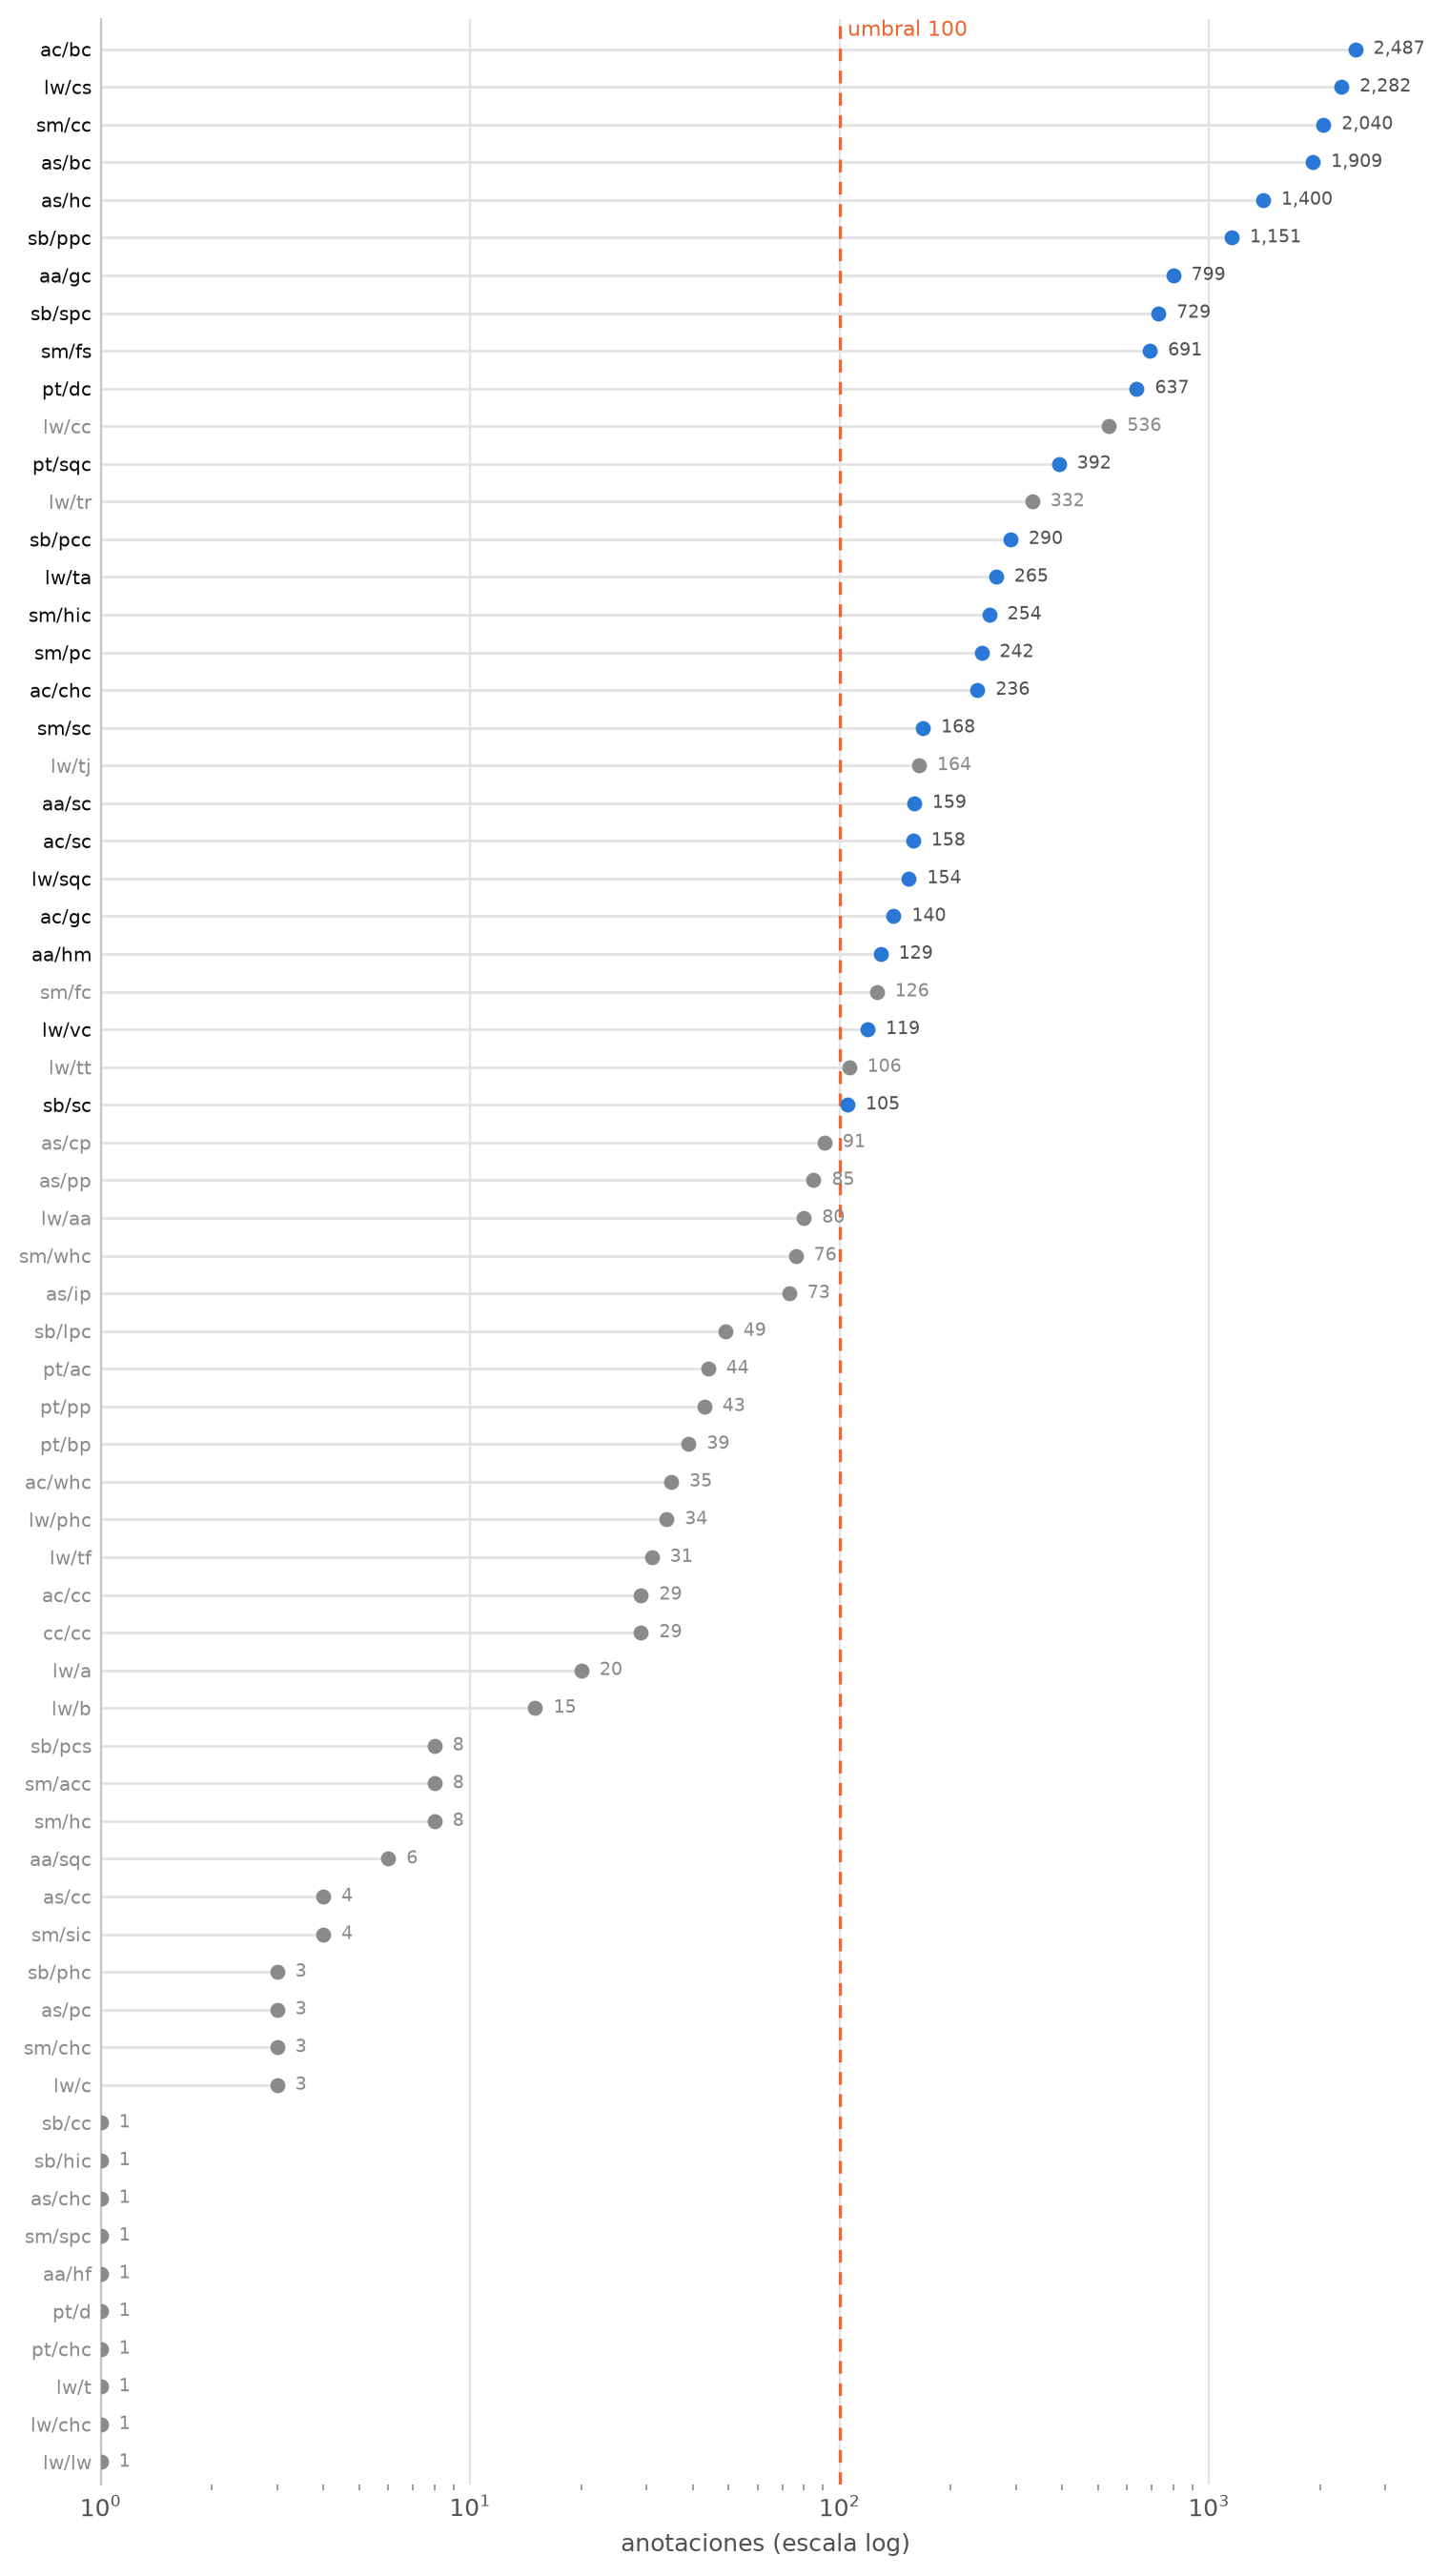
\includegraphics[height=0.80\textheight]{capitulos/04_oe1_curacion/figures/annotations_per_pair.png}
    \caption[Anotaciones por par]{Anotaciones por par de especie y tipo de llamada. Las 25 clases por
        encima del umbral de 100 concentran el 92,5\,\% de las 19\,042 anotaciones;
        la cola larga llega hasta pares con una sola.}
    \label{fig:annotations-per-pair}
\end{figure}

\begin{table}[htbp]
    \centering
    \small
    \begin{threeparttable}
        \caption[Clases del subconjunto de experimento]{Clases del subconjunto de experimento y clases de frase excluidas}
        \label{tab:clases-experimento}
        \begin{tabular}{@{}L{2.2cm}L{5.2cm}rrL{2.6cm}@{}}
            \toprule
            \textbf{Clase}             & \textbf{Tipo de llamada}   & \thead{Anot.}    & \thead{Cajas\\(train)} & \textbf{Rol} \\
            \midrule
            \texttt{ac/bc}             & Ladrido                    & 2\,487           & 2\,886                 & Experimento  \\
            \texttt{lw/cs}             & Sílaba de contacto         & 2\,316           & 2\,706                 & Experimento  \\
            \texttt{sm/cc}             & Llamada de contacto        & 2\,040           & 2\,359                 & Experimento  \\
            \texttt{as/bc}             & Ladrido                    & 1\,909           & 2\,233                 & Experimento  \\
            \texttt{as/hc}             & Aullido                    & 1\,401           & 6\,933                 & Experimento  \\
            \texttt{sb/ppc}            & Llamada de juego           & 1\,151           & 1\,300                 & Experimento  \\
            \texttt{aa/gc}             & Llamada de trago           & 796              & 924                    & Experimento  \\
            \texttt{sb/spc}            & Llamada de escupido        & 730              & 860                    & Experimento  \\
            \texttt{sm/fs}             & Sílaba de comida           & 691              & 801                    & Experimento  \\
            \texttt{pt/dc}             & Dueto                      & 638              & 1\,950                 & Experimento  \\
            \texttt{lw/trino}          & Trino (fusión de 4 tipos)  & 634              & 739                    & Experimento  \\
            \texttt{pt/sqc}            & Chillido                   & 392              & 465                    & Experimento  \\
            \texttt{sb/pcc}            & Llamada de contacto (pío)  & 291              & 342                    & Experimento  \\
            \texttt{lw/ta}             & Alarma terrestre           & 266              & 312                    & Experimento  \\
            \texttt{sm/hic}            & Llamada \textit{hip}       & 254              & 295                    & Experimento  \\
            \texttt{sm/pc}             & Ronroneo                   & 242              & 283                    & Experimento  \\
            \texttt{ac/chc}            & Parloteo                   & 232              & 276                    & Experimento  \\
            \texttt{sm/sc}             & Chillido                   & 168              & 200                    & Experimento  \\
            \texttt{aa/sc}             & Chirrido                   & 159              & 183                    & Experimento  \\
            \texttt{ac/sc}             & Chirrido                   & 158              & 188                    & Experimento  \\
            \texttt{lw/sqc}            & Chillido                   & 155              & 182                    & Experimento  \\
            \texttt{ac/gc}             & Gruñido                    & 140              & 191                    & Experimento  \\
            \texttt{aa/hm}             & Ululato                    & 129              & 148                    & Experimento  \\
            \texttt{lw/vc}             & Contacto visual            & 121              & 140                    & Experimento  \\
            \texttt{sb/sc}             & Alarido                    & 105              & 126                    & Experimento  \\
            \midrule
            \texttt{lw/cc}             & Llamada de contacto        & 517              & ---                    & Excluida: contiene sílabas \\
            \texttt{sm/fc}             & Llamada de comida          & 126              & ---                    & Excluida: contiene sílabas \\
            \texttt{sb/pcs}            & Secuencia de píos          & 8                & ---                    & Excluida: contiene sílabas \\
            \midrule
            \textbf{Total experimento} &                            & \textbf{17\,605} & \textbf{27\,022}       &              \\
            \bottomrule
        \end{tabular}
        \begin{tablenotes}[flushleft]
            \footnotesize
            \item Las tres clases de frase se retiran por anidamiento
            (sección~\ref{sec:silabas}), no por escasez: \texttt{lw/cc} supera
            holgadamente el umbral y habría entrado al experimento.
            \item La columna de cajas cuenta ventanas de 3\,s de la partición de
            entrenamiento, no anotaciones. Las dos cifras no son proporcionales:
            \texttt{as/hc} y \texttt{pt/dc} multiplican su material porque cada
            llamada larga atraviesa varias ventanas
            (sección~\ref{sec:ventaneo}), y son las dos únicas clases donde eso
            ocurre.
        \end{tablenotes}
    \end{threeparttable}
\end{table}

\section{Conjunto acústico curado y particionado (RE1.2)}
\label{sec:re12}
\label{sec:ventaneo}

\subsection{Partición por archivo de grabación}

El conjunto se divide en entrenamiento, validación y prueba en proporción
60/22,5/17,5 de cajas por clase, con semilla fijada para que la partición sea
reproducible. La asignación es golosa y recorre las clases de la más rara a la
más común, de modo que el reparto de las clases escasas se decide primero y no
queda como residuo del de las abundantes. El resultado son 21\,966 ventanas de
entrenamiento, 9\,446 de validación y 8\,007 de prueba, con 27\,022, 10\,090 y
7\,985 cajas anotadas respectivamente. La división
se hace \textbf{por archivo de grabación}: todas las anotaciones de una misma
grabación caen en la misma partición, y ninguna ventana cruza particiones.

La alternativa de repartir anotaciones o ventanas sueltas no es un descuido
hipotético. El prototipo inicial de este trabajo la cometió: barajaba los clips
de 0,5\,s y los repartía por índice, con lo que dos ventanas solapadas
procedentes de la misma anotación podían quedar una en entrenamiento y otra en
prueba. Sobre esa partición el clasificador alcanzaba un 99\,\% de exactitud, una
cifra que no medía generalización sino memoria: el 91,2\,\% de los clips eran
negativos, de modo que un predictor constante ``sin llamada'' ya obtenía 91,2\,\%.
Dado que la variación en las etiquetas fuertes afecta por sí sola a la evaluación
\citep{koga_lead_2024}, no añadir además fuga de datos es la condición mínima
para que las cifras resulten interpretables.

La Tabla~\ref{tab:split} recoge la composición resultante.

\begin{table}[htbp]
    \centering
    \small
    \begin{threeparttable}
        \caption{Composición de las particiones tras el ventaneo}
        \label{tab:split}
        \begin{tabular}{@{}L{3.2cm}rrr@{}}
            \toprule
            \textbf{Partición} & \thead{Grabaciones} & \thead{Ventanas} & \thead{Cajas}    \\
            \midrule
            Entrenamiento      & 1\,166              & 8\,022           & 16\,674          \\
            Validación         & 166                 & 1\,043           & 2\,183           \\
            Prueba             & 335                 & 2\,490           & 5\,343           \\
            \midrule
            \textbf{Total}     & \textbf{1\,667}     & \textbf{11\,555} & \textbf{24\,200} \\
            \bottomrule
        \end{tabular}
        \begin{tablenotes}[flushleft]
            \footnotesize
            \item Hay más cajas que anotaciones porque una misma anotación puede
            caer en dos ventanas consecutivas: la ventana de 3\,s avanza 1,5\,s.
        \end{tablenotes}
    \end{threeparttable}
\end{table}

El balance entre clases se conserva a lo largo de las tres particiones, con un
rango de cajas de entrenamiento que va de 3\,273 para \texttt{lw/cs} a 320 para
\texttt{as/hc}. Ese último número llama la
atención: \texttt{as/hc} tiene 1\,400 anotaciones en la
Tabla~\ref{tab:clases-experimento} y, sin embargo, aporta menos cajas que clases
con la mitad de anotaciones. La razón es estructural y se documenta a
continuación.


\begin{figure}[htbp]
    \centering
    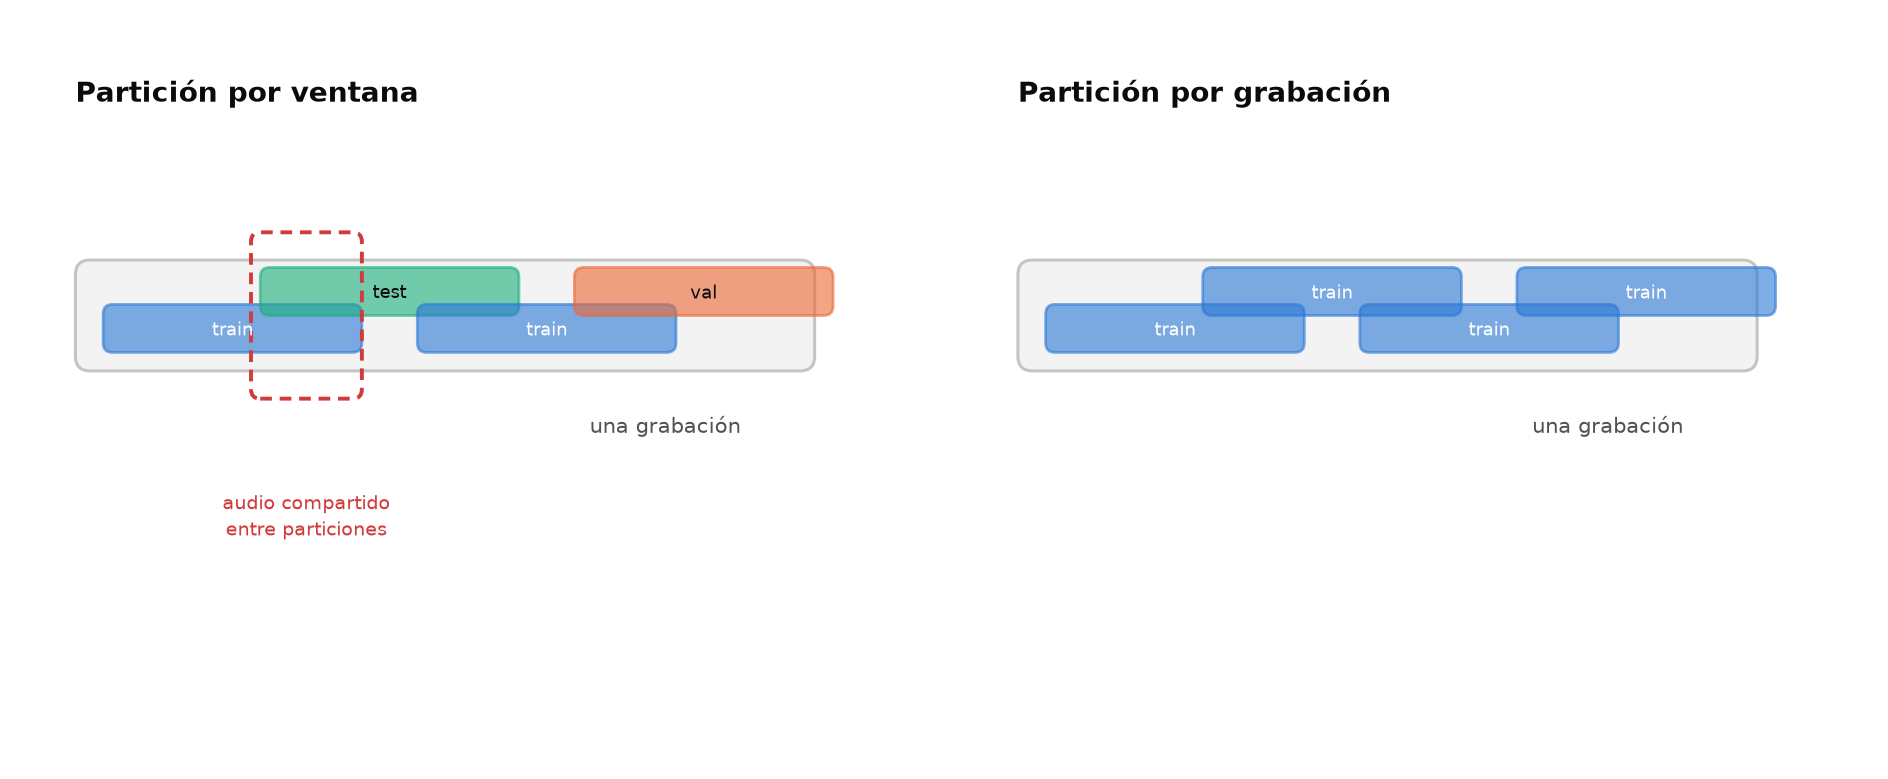
\includegraphics[width=\textwidth]{capitulos/04_oe1_curacion/figures/split_by_recording.png}
    \caption{Partición por grabación.}
    \label{fig:split-by-recording}
\end{figure}

\subsection{El ventaneo y lo que le cuesta a las llamadas largas}

Las grabaciones tienen duración variable y el detector consume entradas de tamaño
fijo, de modo que cada grabación se segmenta en ventanas de 3\,s que avanzan
1,5\,s. La regla de asignación no compara el solapamiento contra la duración del
evento sino contra su \emph{parte visible}, definida como el mínimo entre la
duración del evento y la longitud de la ventana: una anotación entra en una
ventana si el solapamiento cubre al menos la mitad de esa parte visible.

El detalle no es menor. Comparar contra la duración completa dejaría
\textbf{inalcanzable a todo evento de más de 6\,s}, porque no existe posición de
la ventana en la que quepa la mitad de un aullido de 30\,s; con el criterio de
parte visible, en cambio, ese aullido entra en toda ventana que caiga dentro de
él. Ninguna anotación del subconjunto de experimento queda sin ventana.

Lo que el ventaneo cobra es otra cosa, y la Tabla~\ref{tab:ventaneo-largos} la
mide: las llamadas largas se \textbf{fragmentan}. Cada evento se reparte, en
promedio, entre 2,6 ventanas —consecuencia directa del salto de 1,5\,s, que hace
que casi todo evento breve aparezca en dos—, pero \texttt{as/hc} se reparte entre
8,2 y \texttt{pt/dc} entre 5,1. El aullido de \texttt{as/hc}, con 1\,401
anotaciones, aporta 11\,557 cajas: el 26\,\% de todas las cajas del conjunto
derivado provienen del 8\,\% de las anotaciones. Y esas cajas no son recortes
cualesquiera: el 99,6\,\% de las de \texttt{as/hc} toca al menos un borde
temporal de su ventana, y en el 78\,\% de los casos la caja ocupa la ventana
entera de lado a lado.

\begin{table}[htbp]
    \centering
    \small
    \begin{threeparttable}
        \caption[Efecto del ventaneo sobre las clases largas]{Efecto del ventaneo de 3\,s sobre las clases de eventos largos}
        \label{tab:ventaneo-largos}
        \begin{tabular}{@{}L{2.2cm}rrrrr@{}}
            \toprule
            \textbf{Clase}    & \thead{Anot.}    & \thead{Cajas}    & \thead{Cajas por\\anotación} & \thead{Anot.\\$>3$\,s} & \thead{Cajas en\\el borde} \\
            \midrule
            \texttt{as/hc}    & 1\,401           & 11\,557          & 8,2                          & 94,6\,\%               & 99,6\,\%                   \\
            \texttt{pt/dc}    & 638              & 3\,249           & 5,1                          & 90,8\,\%               & 99,2\,\%                   \\
            \midrule
            Resto (23 clases) & 15\,566          & 30\,291          & 1,9                          & 0,3\,\%                & 11,8\,\%                   \\
            \midrule
            \textbf{Total}    & \textbf{17\,605} & \textbf{45\,097} & \textbf{2,6}                 & \textbf{11,1\,\%}      & \textbf{40,6\,\%}          \\
            \bottomrule
        \end{tabular}
        \begin{tablenotes}[flushleft]
            \footnotesize
            \item Una caja está ``en el borde'' cuando su lado temporal
            izquierdo o derecho coincide con el límite de la ventana, es decir,
            cuando el evento continúa fuera de ella.
        \end{tablenotes}
    \end{threeparttable}
\end{table}

Esto se documenta aquí, y no en el apartado de limitaciones, porque determina la
lectura de los resultados por clase del Capítulo~\ref{cap:deteccion} en dos
direcciones opuestas. Por un lado, \texttt{as/hc} y \texttt{pt/dc} se vuelven las
clases \emph{más fáciles} del conjunto: una caja que ocupa la ventana completa se
acierta con casi cualquier predicción grande, y los cuatro modelos evaluados
recuperan entre el 88 y el 95\,\% de las cajas de \texttt{as/hc} y entre el 70 y el
82\,\% de las de \texttt{pt/dc}, muy por encima de lo que obtienen en cualquier
otra clase de tamaño comparable. Por otro, al aportar el 33\,\% de
las cajas, esas dos clases dominan cualquier cifra agregada: un \textit{recall}
global que las incluya mide, en un tercio de su peso, la capacidad de dibujar un
rectángulo del tamaño de la ventana. Por eso el Capítulo~\ref{cap:deteccion}
reporta el promedio por clase junto al agregado, y no en su lugar.

Es, además, la manifestación concreta del rango de 2\,134$\times$ en duración de
la Tabla~\ref{tab:geometria}: una ventana única no puede a la vez resolver un
chirrido de 34\,ms y contener un aullido de 73\,s. Una segunda longitud de
ventana para las clases largas, o una etapa de agregación que reconstruya el
evento completo a partir de sus fragmentos antes de puntuarlo, sigue siendo el
principal pendiente de esta etapa.

\begin{figure}[htbp]
    \centering
    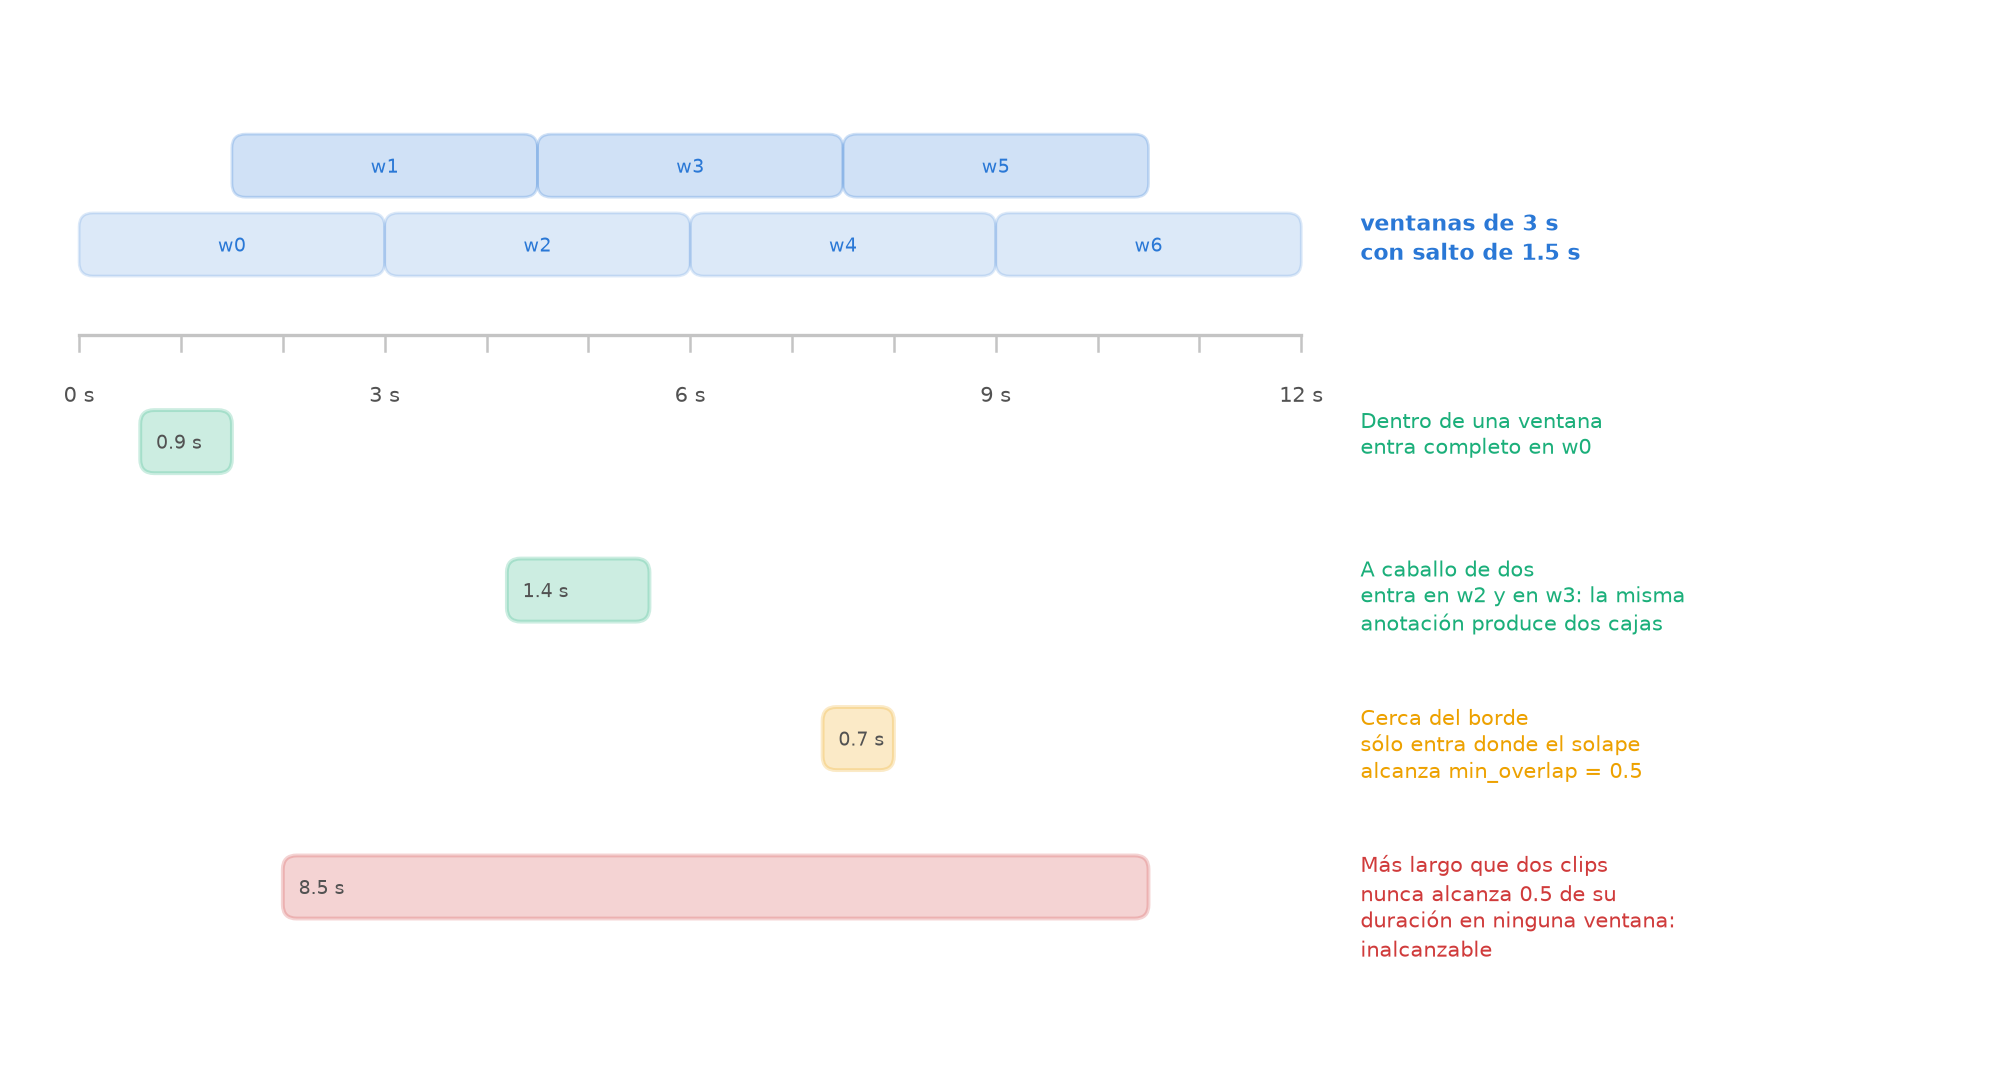
\includegraphics[width=\textwidth]{capitulos/04_oe1_curacion/figures/windowing.png}
    \caption{Efecto del ventaneo.}
    \label{fig:windowing}
\end{figure}

\subsection{Densidad de eventos por ventana}

Conviene registrar cuántas anotaciones coinciden en una misma ventana de 3\,s: la
mediana es 1 y el máximo observado, 11; el 97\,\% de las ventanas con contenido
lleva cuatro cajas o menos. Es una propiedad del conjunto derivado, pero se
consigna aquí porque el Capítulo~\ref{cap:deteccion} la usa para dimensionar el
número de predicciones simultáneas que el decodificador debe sostener: el
presupuesto se fija sobre el máximo y no sobre la mediana.

A las ventanas con al menos una anotación se suma un 25\,\% de ventanas
\emph{vacías} tomadas al azar de tramos sin ninguna llamada. Sin ellas el modelo
nunca ve fondo puro —selva, lluvia, insectos— y aprende que en toda entrada hay
algo que reportar, que es exactamente el sesgo que la carga de revisión paga.


\subsection{Representación y normalización de las cajas}

Cada ventana se transforma en un espectrograma log-mel con los parámetros de la
Tabla~\ref{tab:preproc}. Log-mel es la representación con la que se materializa
el caché, y la que consumen las tres arquitecturas; la normalización de energía
por canal anunciada en la sección~\ref{sec:representacion} no la reemplaza sino
que se aplica encima, como capa entrenable de entrada de la arquitectura
propuesta (sección~\ref{sec:arquitectura}). La ablación que la compara contra la
compresión logarítmica fija está implementada en el repositorio, pero todavía no
medida. La columna de justificación registra qué falla con el
ajuste alternativo, que es la información que permite revisar un parámetro sin
repetir el experimento que lo fijó. La tabla reúne los once parámetros que
fijan el espectrograma de principio a fin —del remuestreo de la señal a la
compresión logarítmica final—, de modo que reproducirlo no exige leer el
código: basta con \texttt{torchaudio.transforms.MelSpectrogram} instanciada con
estos valores (\texttt{src/core/config.py} y \texttt{src/utils/audio.py}).

\begin{table}[htbp]
    \centering
    \caption[Parámetros de preprocesamiento]{Parámetros de preprocesamiento y motivo de cada elección}
    \label{tab:preproc}
    \small
    \begin{tabular}{@{}L{2.6cm}L{3.0cm}L{8.3cm}@{}}
        \toprule
        \textbf{Parámetro}       & \textbf{Valor}        & \textbf{Justificación} \\
        \midrule
        Frecuencia de muestreo   & 44\,100\,Hz           &
        Igual a la de las grabaciones primarias, de modo que esta etapa no
        remuestrea; su mitad --22\,050\,Hz-- es el techo de Nyquist que fija el
        límite superior del rango de frecuencia más abajo                        \\
        \addlinespace
        Ventana / salto          & 3,0\,s / 1,5\,s       &
        Contiene entera a 23 de las 25 clases; el costo es la fragmentación de
        las dos largas (Tabla~\ref{tab:ventaneo-largos})                          \\
        \addlinespace
        Solapamiento mínimo      & 0,5                   &
        Un evento entra en una ventana si la mitad de su parte visible cae
        dentro; medirlo contra la parte visible y no contra la duración total
        es lo que mantiene alcanzables a los eventos de más de 6\,s               \\
        \addlinespace
        Longitud de ventana STFT & 1\,024 (23\,ms)       &
        Más corta que los eventos más breves: 34\,ms el mínimo, 81\,ms la mediana
        de \texttt{sm/cc}                                                         \\
        \addlinespace
        Función de ventana       & Hann                  &
        Valor por defecto de \texttt{torchaudio}; no se exploró una alternativa
        porque ninguna clase mostró fuga espectral atribuible a la ventana       \\
        \addlinespace
        Puntos de la FFT         & 4\,096                &
        Relleno con ceros: densifica la rejilla de frecuencia sin tocar la
        resolución temporal                                                       \\
        \addlinespace
        Salto STFT               & 400 (9\,ms)           &
        Produce 331 tramas por ventana                                            \\
        \addlinespace
        Bandas mel               & 128                   &
        Lo que espera el extractor preentrenado; 256 no dio ganancia medible      \\
        \addlinespace
        Escala mel               & HTK ($q=2\,595$,\newline $f_\text{quiebre}=700$\,Hz) &
        Convención por defecto de \texttt{torchaudio} frente a la alternativa
        Slaney; es la misma fórmula que fija el eje de la
        sección~\ref{sec:representacion}, $m(f) = q \log_{10}(1 + f / f_\text{quiebre})$ \\
        \addlinespace
        Rango de frecuencia      & 25\,Hz -- 22\,050\,Hz &
        Un techo de 16\,kHz truncaba la mitad de las cajas de \texttt{sb/spc},
        cuya frecuencia superior media es 16\,110\,Hz                             \\
        \addlinespace
        Compresión               & $10 \log_{10}(\text{mel} + \epsilon)$,\newline $\epsilon = 10^{-6}$ &
        Espectrograma de potencia ($|\cdot|^2$, no magnitud), de ahí el factor
        10 y no 20; $\epsilon$ evita $-\infty$ en las celdas sin energía         \\
        \bottomrule
    \end{tabular}
\end{table}

Las cajas se normalizan al formato de centro, ancho y alto en el intervalo
$[0,1]$, con el eje de frecuencia mapeado a través de la misma escala mel que
produce la imagen. La consecuencia es que una caja significa lo mismo en el
espacio de píxeles que sobre la pantalla del analista: el rectángulo que el
modelo predice es directamente el rectángulo que Raven dibuja, sin
reinterpretación. La Figura~\ref{fig:window-example} muestra una ventana de
entrenamiento tal como el modelo la recibe.

\begin{figure}[htbp]
    \centering
    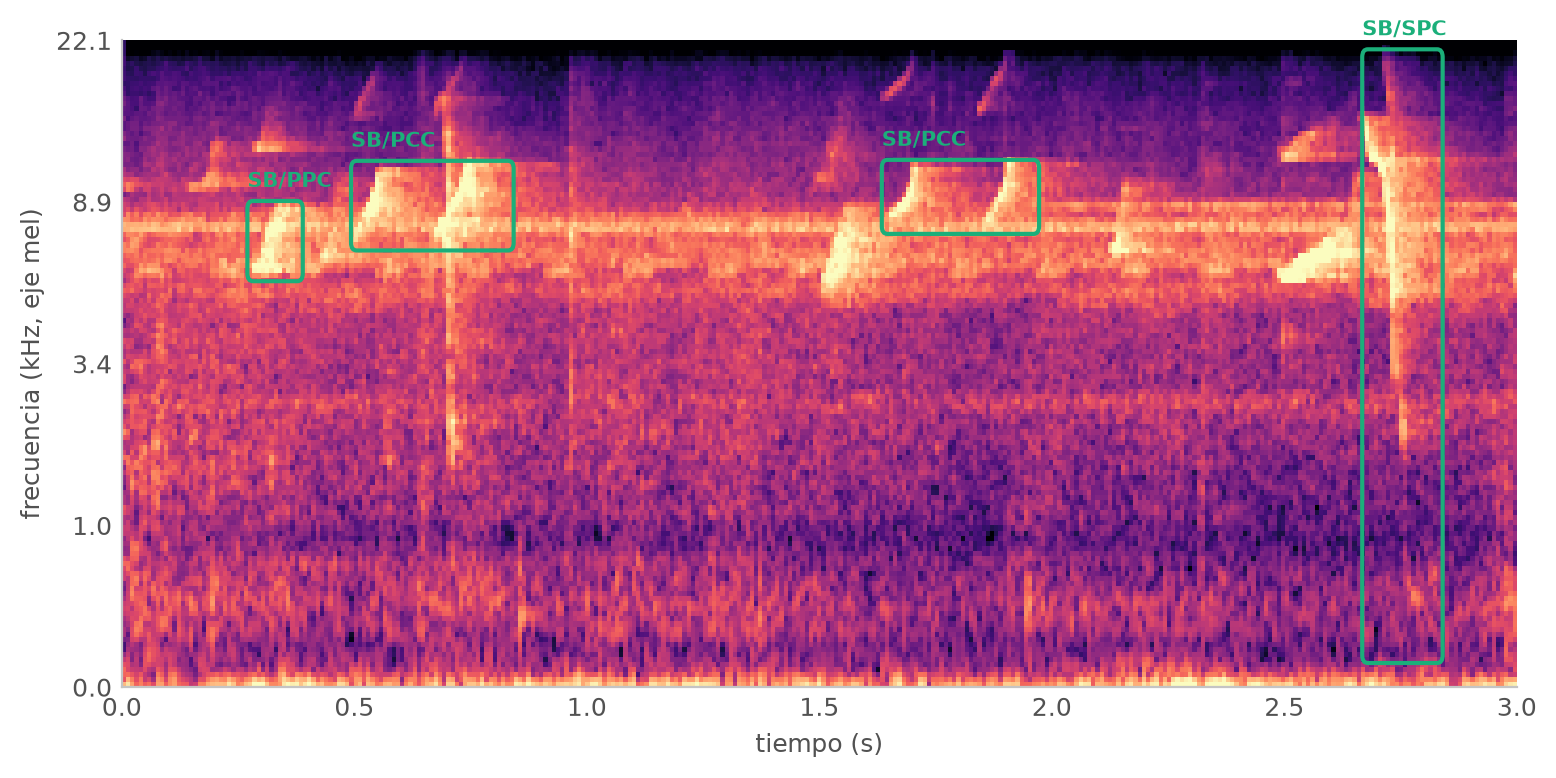
\includegraphics[width=\textwidth]{capitulos/04_oe1_curacion/figures/window_example.png}
    \caption[Ventana de entrenamiento]{Una ventana de entrenamiento: espectrograma log-mel de 3\,s con los
        parámetros de la Tabla~\ref{tab:preproc} y las cajas objetivo superpuestas
        en el marco normalizado. Las once cajas \texttt{sb/spc} de este clip son el
        caso más denso observado en todo el conjunto.}
    \label{fig:window-example}
\end{figure}

\begin{figure}[htbp]
    \centering
    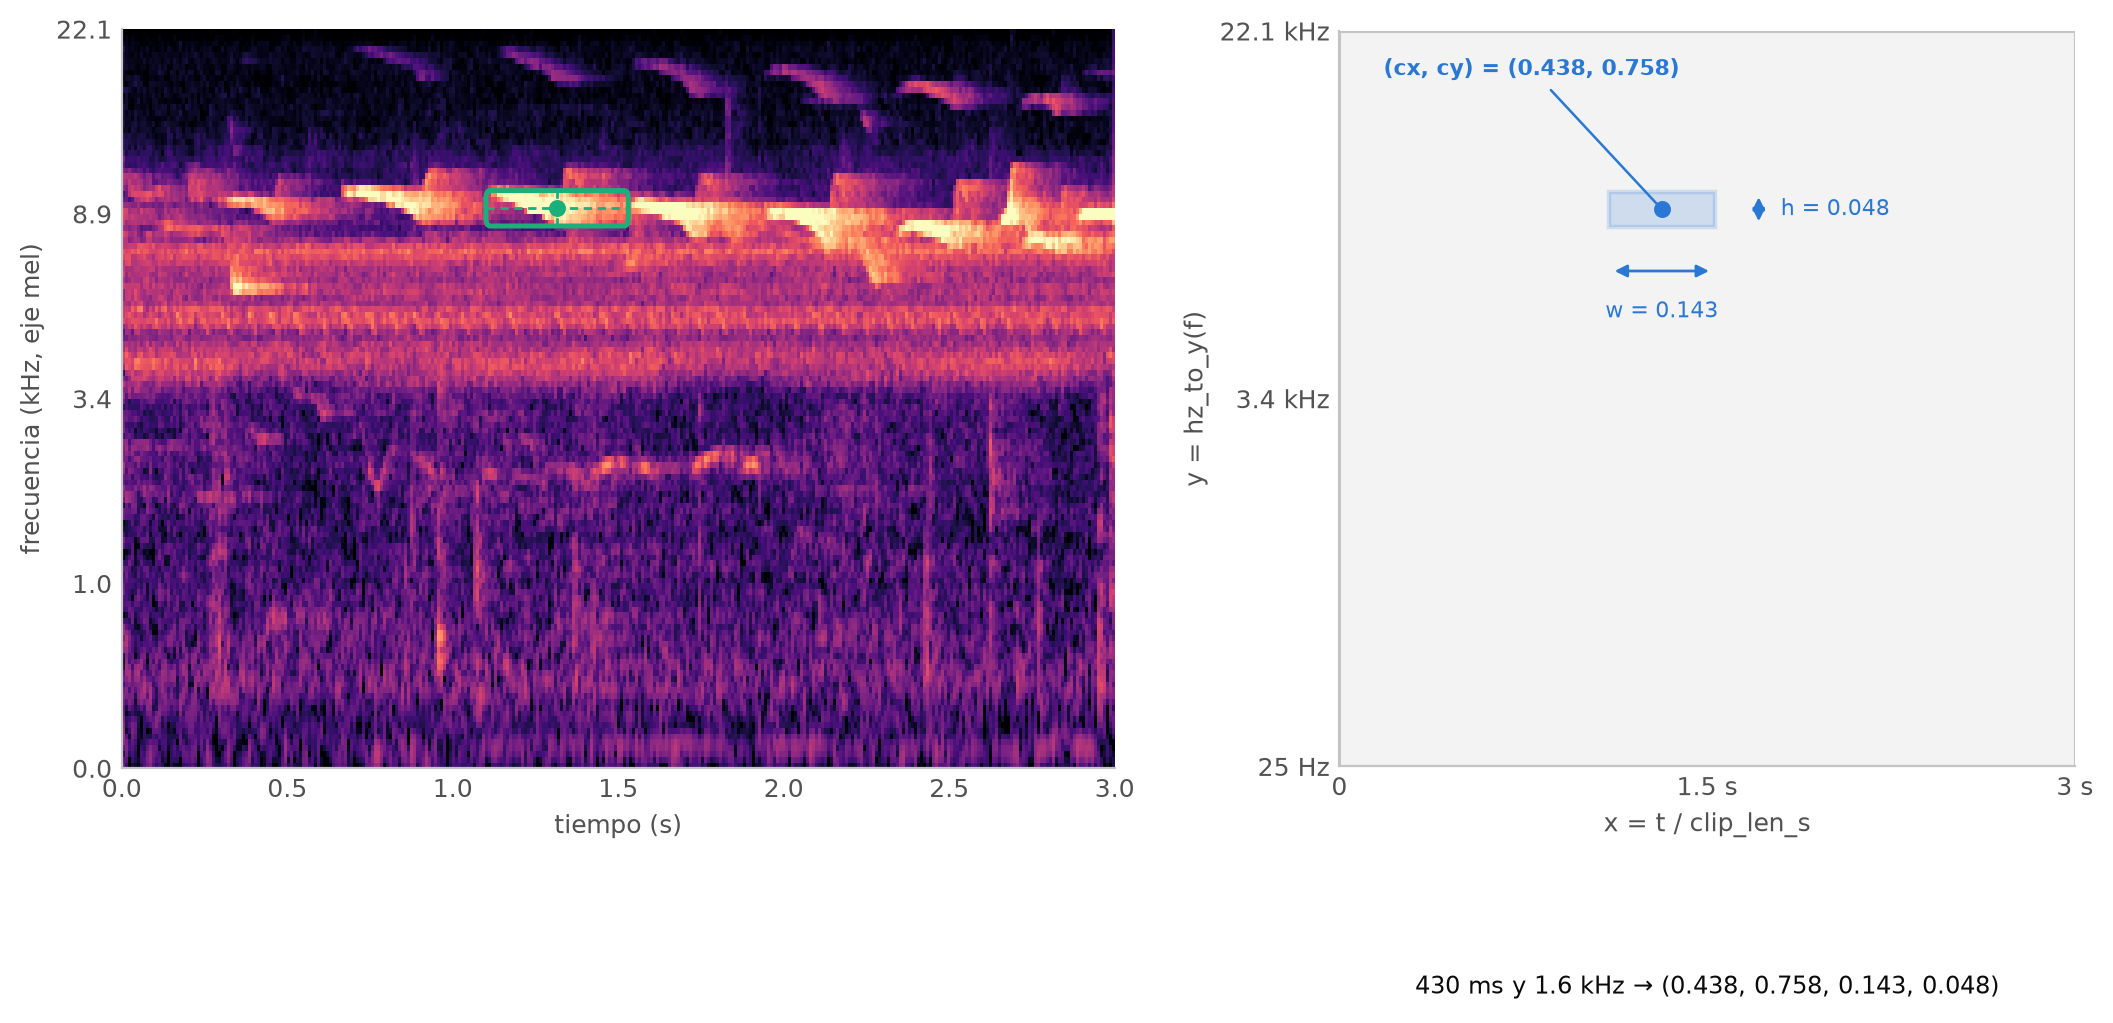
\includegraphics[width=\textwidth]{capitulos/04_oe1_curacion/figures/box_coordinates.png}
    \caption{Coordenadas de la caja.}
    \label{fig:box-coordinates}
\end{figure}

\section{Balance del conjunto de experimento}
\label{sec:revision}

Las 25 clases seleccionadas cubren el 92,5\,\% del material curado, pero la
selección no corrige las dos causas estructurales que este capítulo documentó, y
conviene dejar dicho qué queda en pie antes de leer los resultados del
Capítulo~\ref{cap:deteccion}.

\rotulo{El desbalance no desaparece: se traslada.} Entre \texttt{ac/bc}, la clase
mayoritaria una vez descontada la fragmentación de \texttt{as/hc}, con 2\,886
cajas de entrenamiento, y \texttt{sb/sc}, con 126, median más de veinte veces, y el orden de magnitud se mantiene aunque el umbral baje o suba
(Figura~\ref{fig:boxes-split}). La partición sí preserva el balance: cada clase
conserva aproximadamente la misma proporción en las tres particiones, que es lo
que permite comparar el desempeño por clase entre validación y prueba sin
atribuir a la arquitectura una diferencia de composición.

\begin{figure}[htbp]
    \centering
    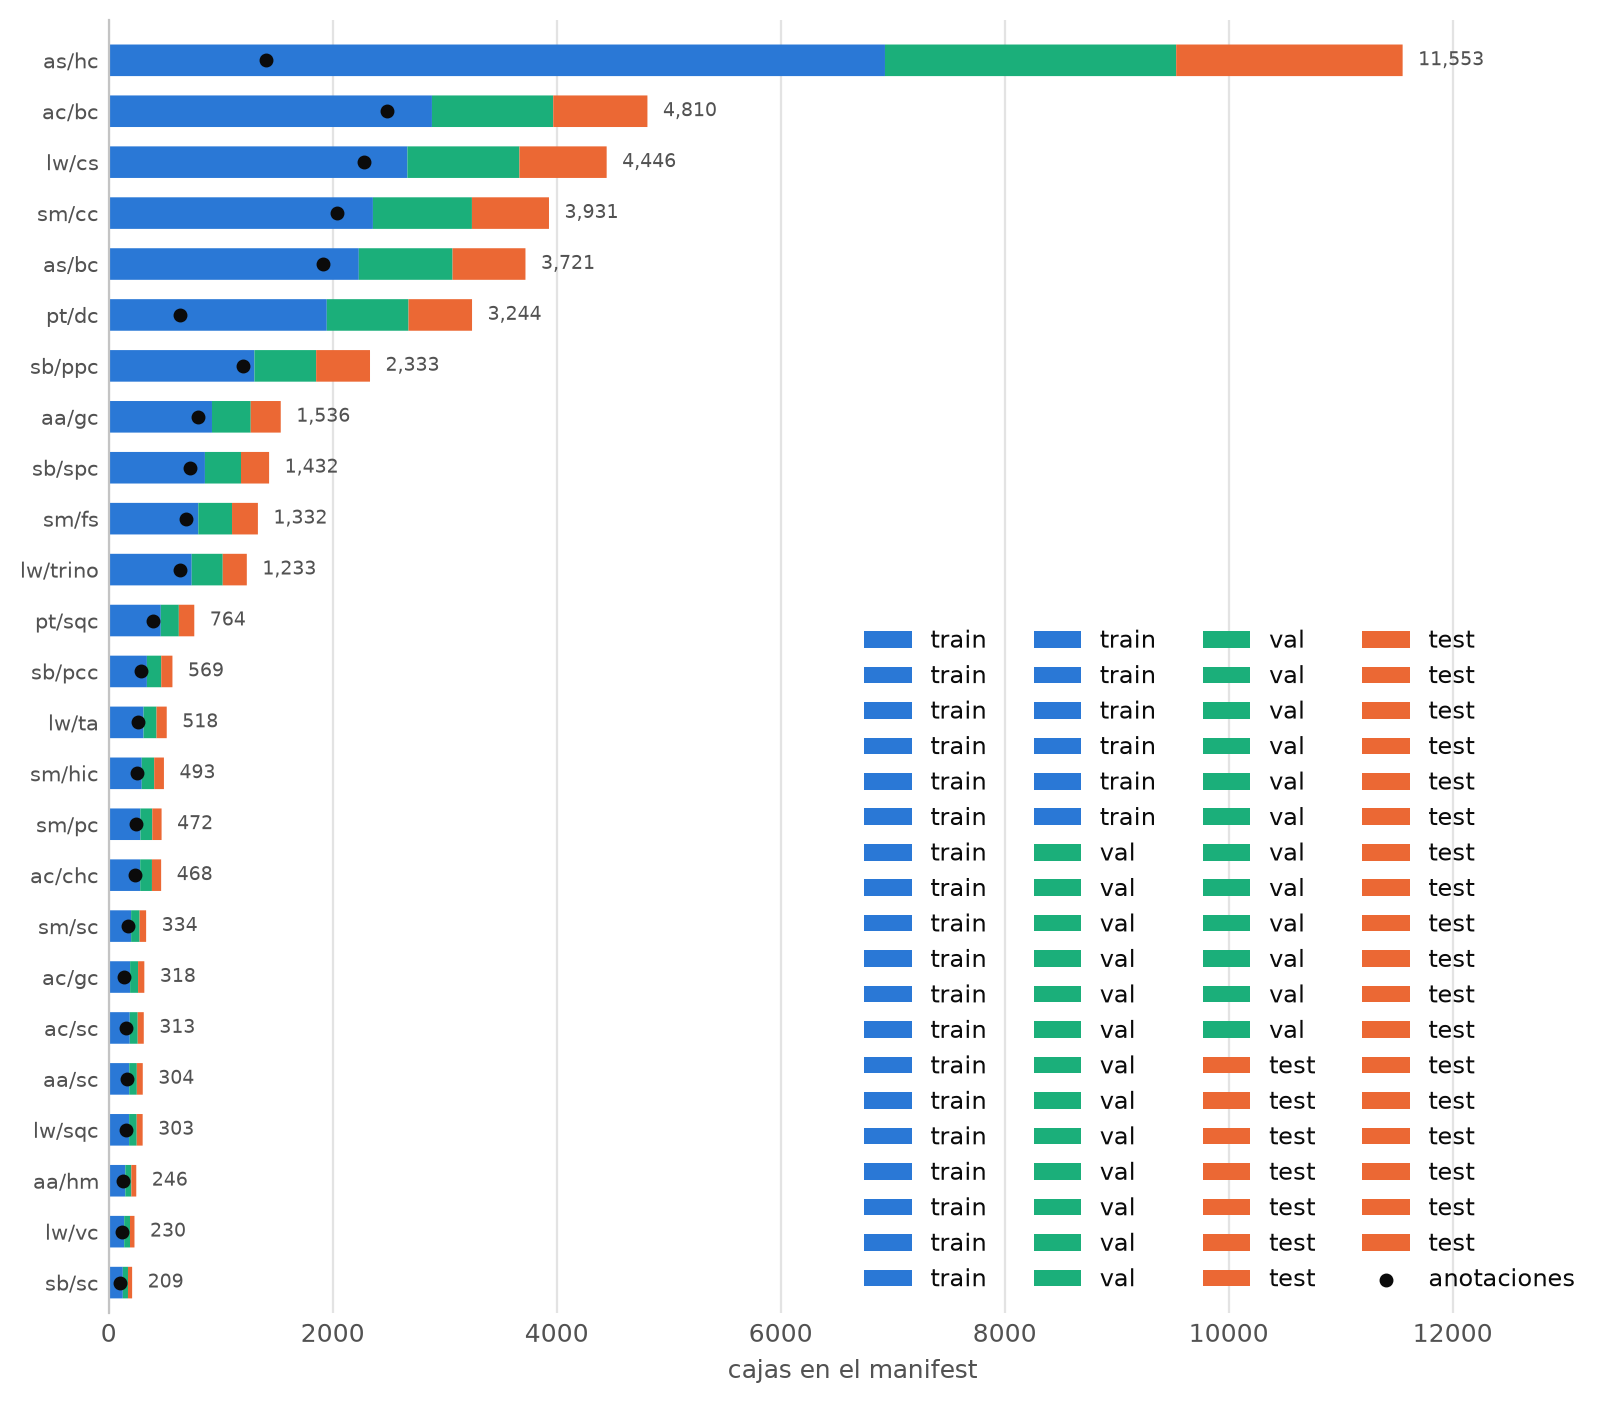
\includegraphics[width=\textwidth]{capitulos/04_oe1_curacion/figures/boxes_per_split.png}
    \caption[Cajas por clase y partición]{Cajas por clase y partición. El balance se preserva entre
        particiones; el desbalance entre clases se mantiene, con más de un orden de
        magnitud entre la clase mayoritaria y las que apenas superan el umbral.}
    \label{fig:boxes-split}
\end{figure}

\rotulo{La escasez y la arquitectura se confunden en el análisis por clase.}
Once de las veinticinco clases aportan menos de 300 cajas de entrenamiento.
Cuando una de ellas obtiene mal \textit{recall}, la causa puede ser el modelo o
puede ser que nunca vio material suficiente, y el Capítulo~\ref{cap:deteccion}
solo puede separar ambas cosas comparando el comportamiento de las cuatro
arquitecturas sobre la misma clase: una clase que todas fallan por igual es
escasez; una que unas recuperan y otras no es arquitectura.

\rotulo{La densidad por ventana es baja.} La mediana de cajas por ventana de
3\,s es 1 y el máximo 11 (Figura~\ref{fig:boxes-window}). El presupuesto de
predicciones simultáneas del decodificador se dimensiona sobre el máximo, no
sobre la mediana, y las 64 consultas de la arquitectura propuesta lo cubren con
holgura.

\begin{figure}[htbp]
    \centering
    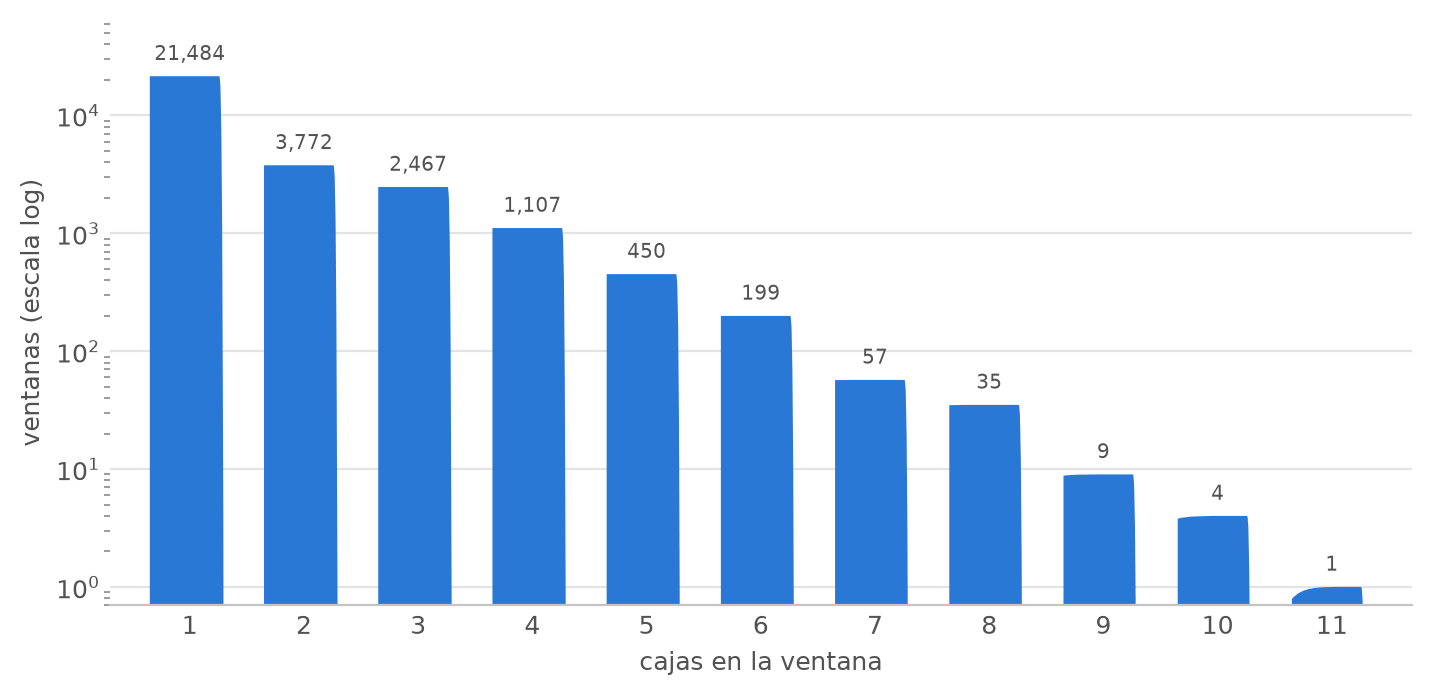
\includegraphics[width=0.92\textwidth]{capitulos/04_oe1_curacion/figures/boxes_per_window.png}
    \caption[Cajas anotadas por ventana]{Cajas anotadas por ventana de 3\,s: mediana 1, máximo 11.}
    \label{fig:boxes-window}
\end{figure}


\section{Ficha del conjunto derivado (RE1.3)}
\label{sec:re13}

La documentación del conjunto sigue la estructura de las \textit{datasheets} para
conjuntos de datos, que proponen registrar motivación, composición, proceso de
recolección, transformaciones aplicadas y usos recomendados, con el propósito de
aumentar la transparencia y la rendición de cuentas \citep{gebru_2021}. La ficha
distingue de forma explícita dos capas de responsabilidad.

\rotulo{Conjunto primario.} Las grabaciones y las anotaciones originales,
producidas por el equipo de investigación. La ficha documenta su origen, el
equipo de captura, la frecuencia de muestreo y el procedimiento de anotación en
Raven, pero no reclama su autoría.

\rotulo{Conjunto derivado.} El resultado de aplicar el protocolo de la
sección~\ref{sec:protocolo}: normalización de etiquetas, vocabulario cerrado,
saneamiento geométrico, selección del subconjunto, partición por archivo de
grabación y ventaneo. Esta capa sí es contribución de esta tesis, y la ficha
registra cada transformación junto con lo que descarta.

La ficha declara además, como limitaciones conocidas del conjunto derivado:

\begin{itemize}[nosep]
    \item La fragmentación de las llamadas largas bajo el ventaneo de 3\,s
          (Tabla~\ref{tab:ventaneo-largos}): \texttt{as/hc} y \texttt{pt/dc} sobreviven
          como series de cajas recortadas al borde de la ventana, y el conjunto no
          incluye ningún mecanismo que las reagrupe en el evento original.
    \item Las tres clases de frase excluidas por anidamiento
          (sección~\ref{sec:silabas}), que dejan sin cubrir el nivel superior de la
          jerarquía vocal.
    \item Los once tipos de llamada en vocabulario que no alcanzan el umbral de
          100 anotaciones (466 registros) y quedan fuera del experimento, entre ellos la
          única clase de CC, que hace que el conjunto de experimento cubra siete
          especies y no ocho.
    \item Los 16 pares fuera de vocabulario (328 registros) pendientes de
          revisión por el equipo de investigación.
    \item Las once clases con menos de 300 cajas de entrenamiento, cuyo
          desempeño individual no puede atribuirse limpiamente a la arquitectura.
    \item La heterogeneidad geométrica de \texttt{ac/bc}, \texttt{sm/fs} y
          \texttt{sb/ppc} (Figura~\ref{fig:facets}), que sugiere etiquetas que agrupan
          variantes distintas de llamada.
    \item La ausencia de una medición de acuerdo entre anotadores, que impide
          separar el error del modelo del techo impuesto por la propia tarea.
\end{itemize}

% TODO Decidir con el equipo si el conjunto se libera y en qué términos.
% Si hay restricciones por ubicación de especies amenazadas, decláralas
% aquí como limitación legítima, no las omitas.

% ===================================================================
\section{Discusión}
\label{sec:discusion-oe1}
% ===================================================================
% TODO Redactar siguiendo las pautas, sin introducir resultados nuevos:
%   (1) resumen de los tres resultados, pasando de las cifras a su lectura
%       descriptiva;
%   (2) qué significan: qué habilita el conjunto derivado y qué decisiones de
%       OE2 quedan condicionadas por su composición y su desbalance;
%   (3) consistencia con la literatura del Capítulo~\ref{cap:estado}: vocabulario
%       cerrado y unidades jerárquicas \citep{kershenbaum_acoustic_2016},
%       fichas de conjunto \citep{gebru_2021}, efecto de la variabilidad de la
%       etiqueta en la evaluación \citep{koga_lead_2024};
%   (4) generalización: qué parte del protocolo sirve para otro corpus de PAM y
%       qué parte es propia de este material;
%   (5) limitaciones: clases de frase excluidas, ausencia de medición de acuerdo
%       entre anotadores y clases con soporte escaso.
% ===================================================================

